%---------------------------------------------------------------------------------------------------
% Realization
%---------------------------------------------------------------------------------------------------
\newpage
%\part{Anfang}
\chapter{Realization}
\label{cap:Realization}
This section keeps the focus on the realization of the Civitas Android application.  
An Android application is a crossplay of Java classes and related .xml files. A Java class contains the programmatical logic, and the .xml file depicts the logic in a graphical frame. The result of the combination is the graphical user interface (GUI).

Therefore, the same user use-cases from the design chapter will be re-introduced from a graphical point of view (see section \ref{design:subsection:use_cases}). To ensure a better understanding and to emphasize the graphical aspect, the order might differ.


\section{Civitas - Android Application}

Now, it is time to put things together and introduce the Civitas app to the user. One can shorten things up by clustering the use-cases. If the user launches the app for the first time, the login screen will be presented. So it is useful to start with user management.

\section{User Management}
As the name indicates, this section deals with user issues. Embedded into the MainActivity the LoginFragment (fig.\ref{fig:login_screen}) is the first screen that appears to the user if he initially launches the Civitas app. Here is the first difference to the old version with its Google Sign-in authentication service. Now, the user has to provide the required data and submit to register (fig. \ref{fig:register_screen}). If the registration is successful, one returns to the Login screen again. 
The last big part of user management is the reset password feature. For resetting the password, the user has to tap at text below the two buttons within the LoginFragment. In order to get reset instructions, one has to fill in the user related email address. It depends on the Backendless user preferences if an email with a temporary password or a link for inserting a new password will be sent. While this document is being written, the second option is selected.
Furthermore, emails were sent for successful registration, and the first login also. These email options can be disabled depending on the product owner preference. During each use-case within the user management, one gets involved in the current process by receive text information and a progress indicator. 

The login screen also has some user assisting features. If the user taps on one of two input fields, the information hint will move upwards. In case of leaving one or two fields empty, the hints get coloured red, and an additional text will inform the user that the fields are mandatory. The little crossed eye at the right end of the password field allows the user to view it as a cleat text. These features will increase the impression of value and the user experience of the \textbf{Civitas} app. 
To simplify the further usage, one stays logged in until the logout button is pressed. The logout button is in the navigation drawer accessible within the MapActivity and the ArtefactActivity.

\begin{figure}[!htb]
\minipage{0.49\textwidth}
  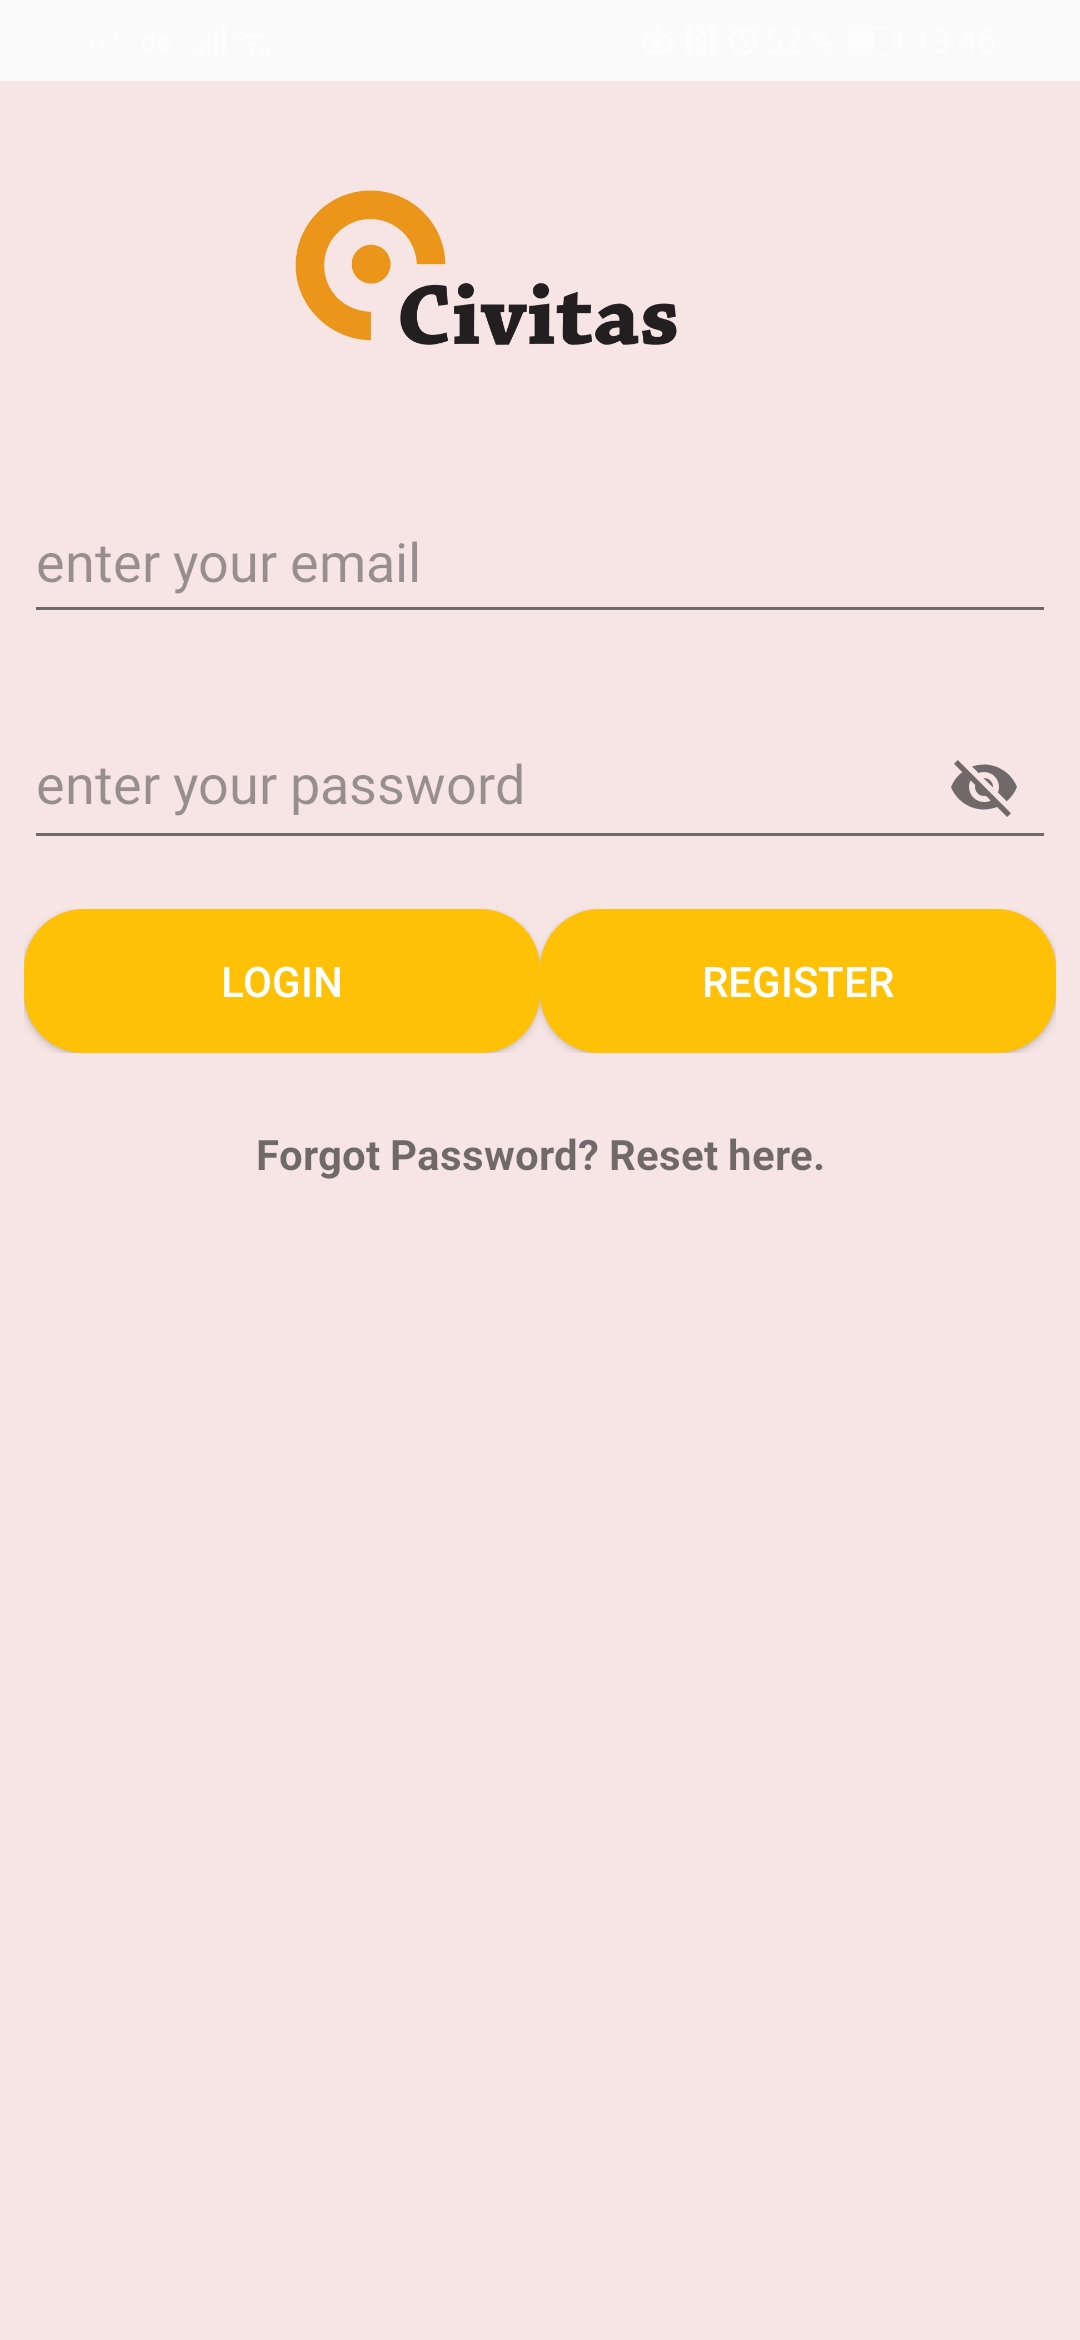
\includegraphics[width=\linewidth]{realization/realization_login.jpg}
  \caption{Login screen}
  \label{fig:login_screen}
\endminipage\hfill
\minipage{0.49\textwidth}
  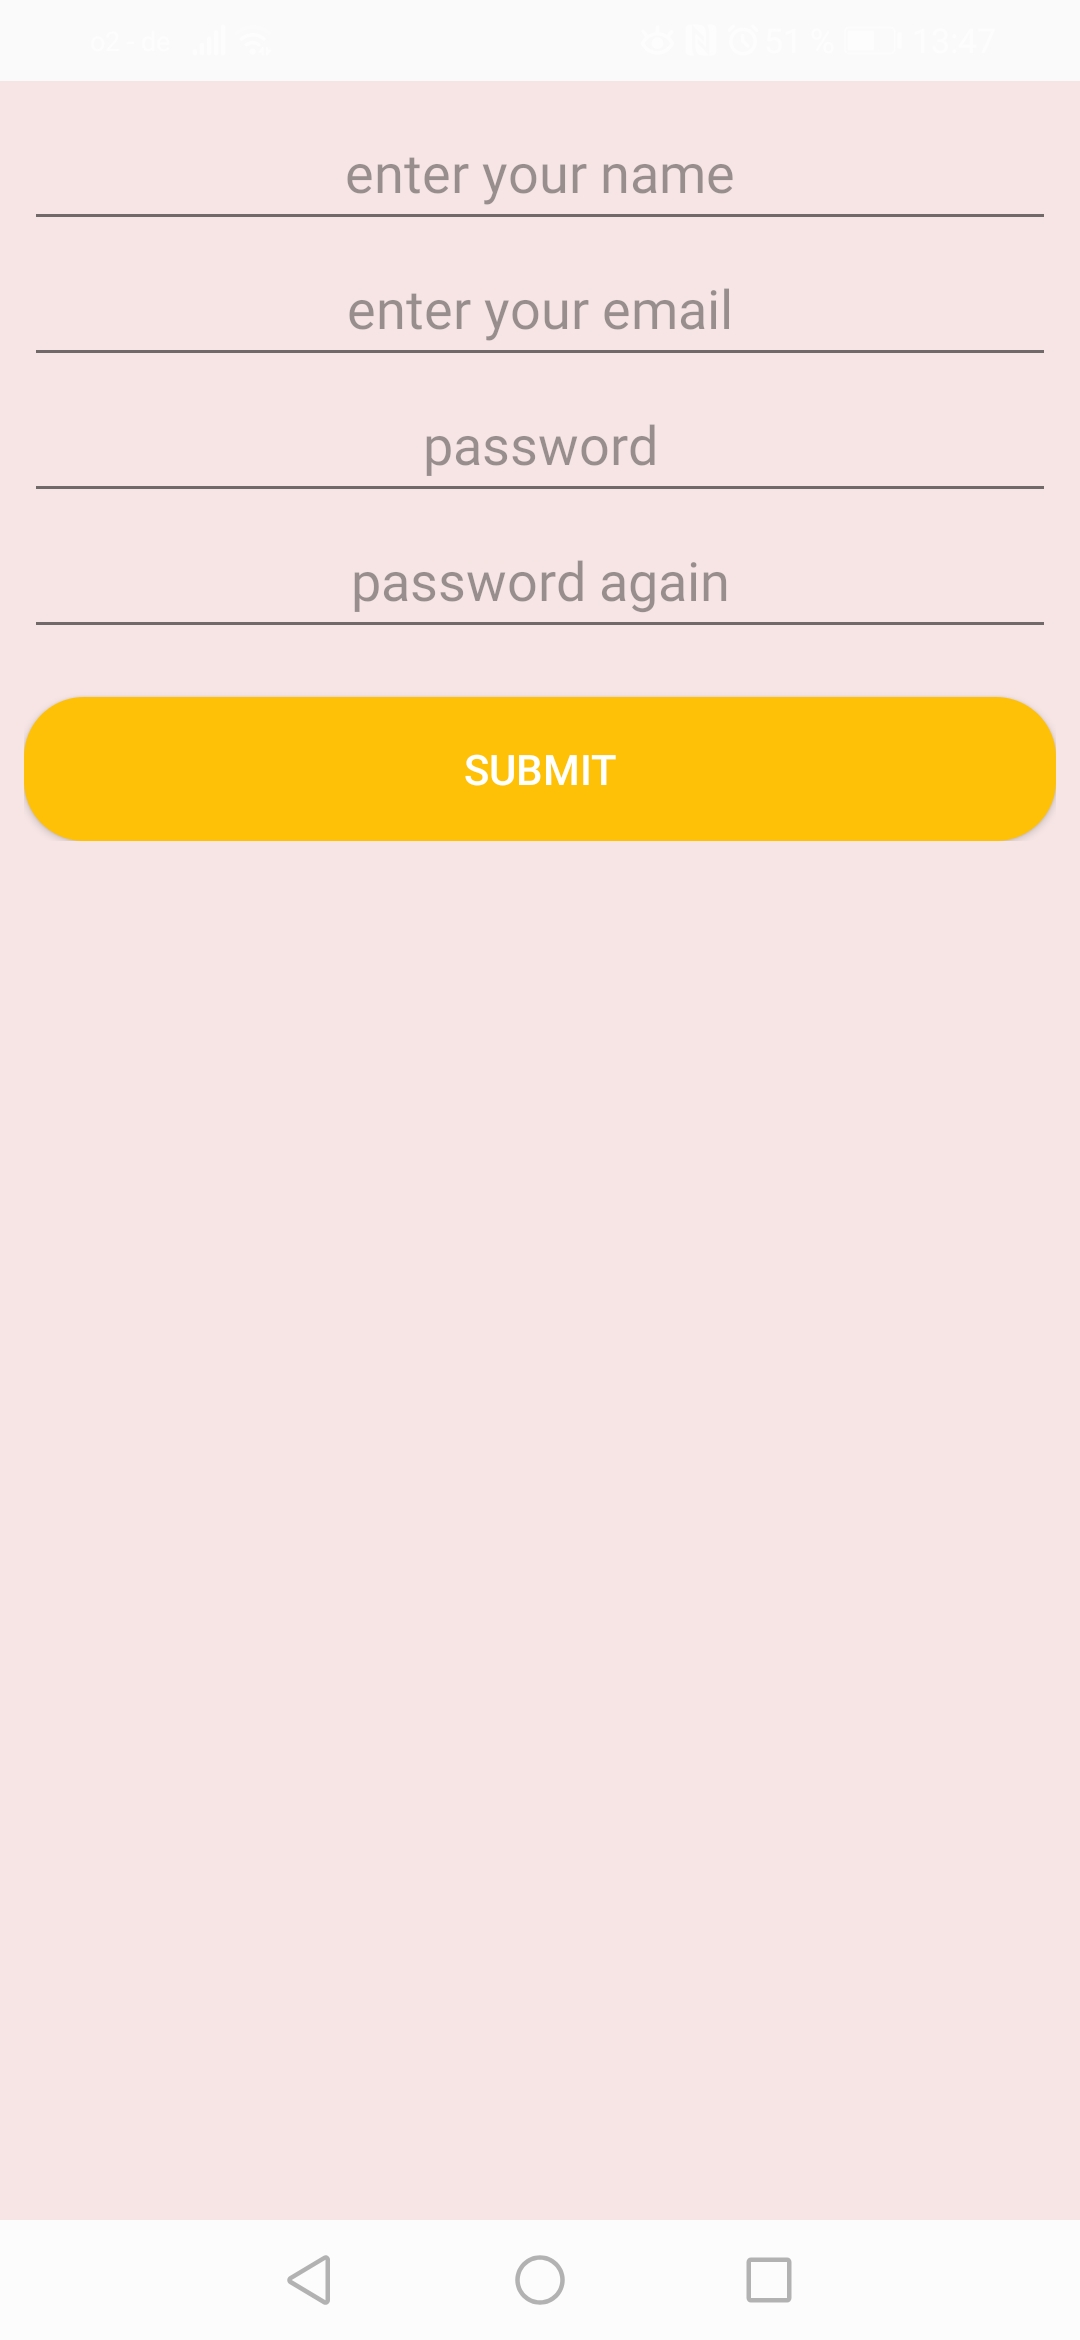
\includegraphics[width=\linewidth]{realization/realization_register.jpg}
  \caption{Register screen}
  \label{fig:register_screen}
\endminipage\hfill
\caption{User management}
\label{fig:user_management}
\end{figure}

\begin{figure}[!htb]
\minipage{0.49\textwidth}
  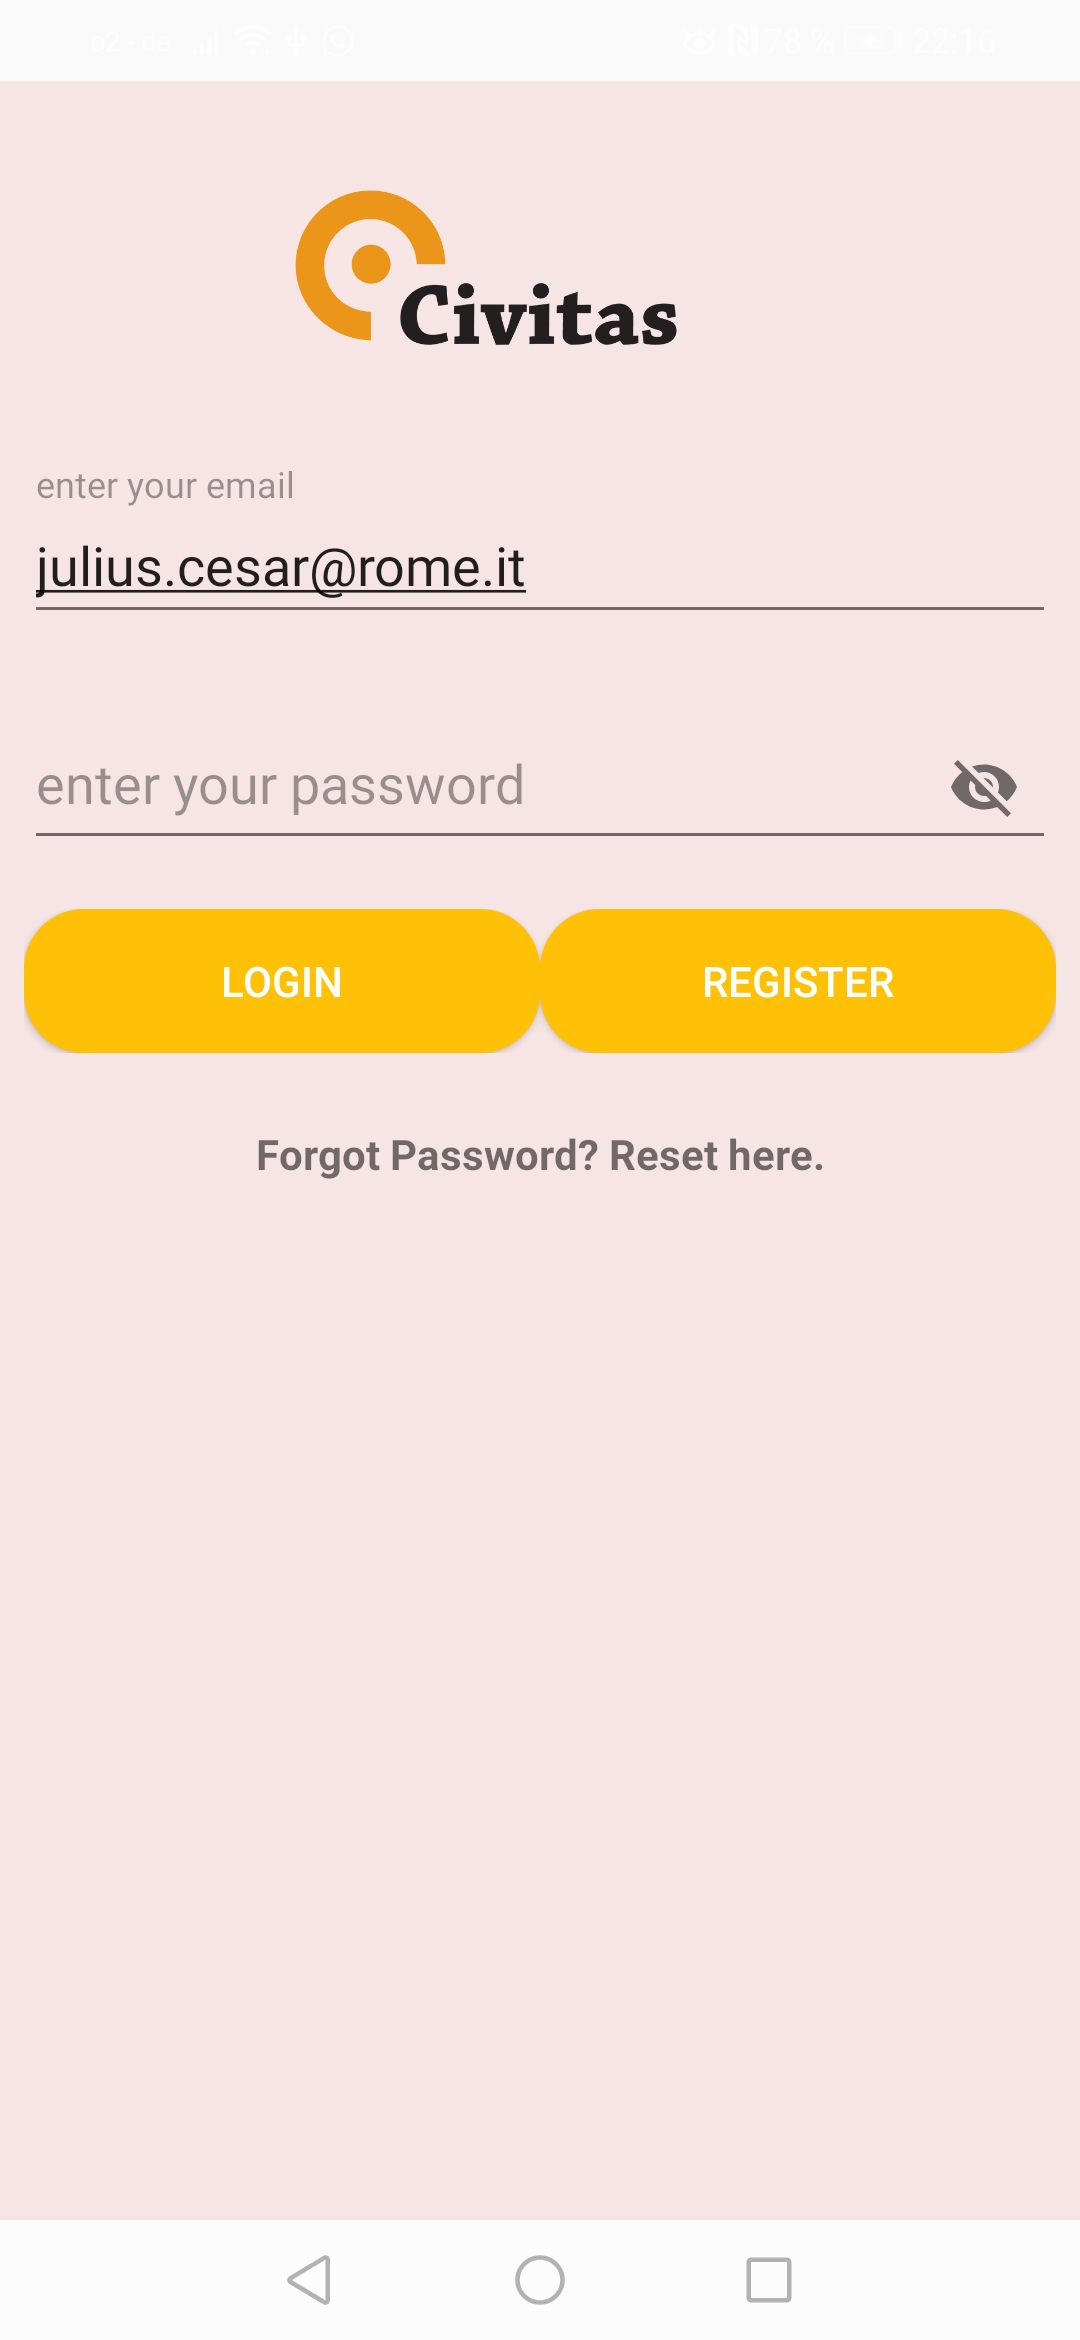
\includegraphics[width=\linewidth]{realization/realization_request_pw.jpg}
  \caption{Request password}
  \label{fig:pw_request}
\endminipage\hfill
\minipage{0.49\textwidth}
  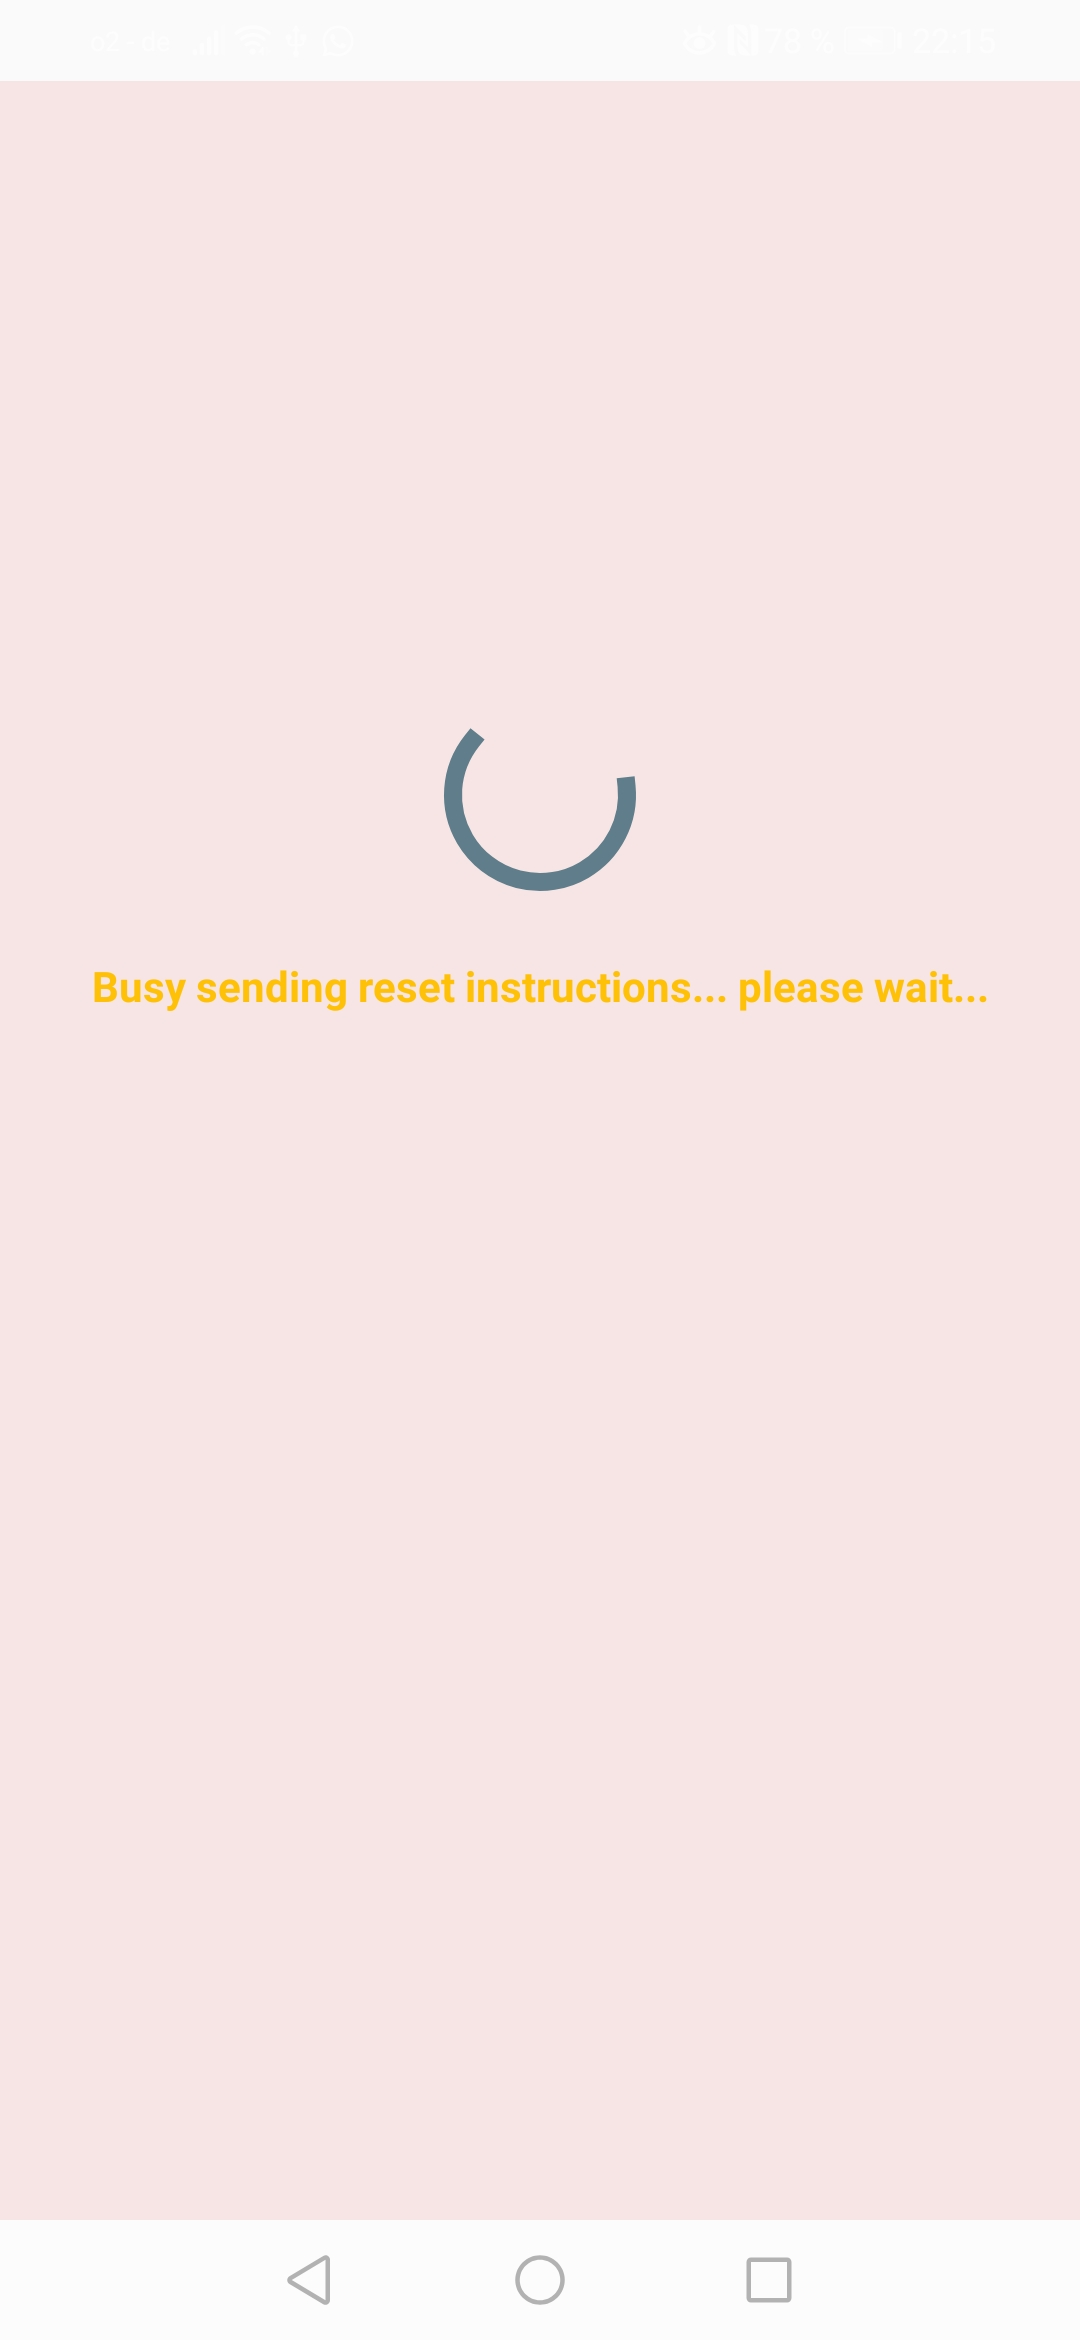
\includegraphics[width=\linewidth]{realization/realization_reset_pw_progress_indicator.jpg}
  \caption{Progress indicator}
  \label{fig:pw_request_progress}
\endminipage\hfill
\caption{Password management}
\label{fig:pw_management}
\end{figure}

\begin{figure}[!htb]
\minipage{0.49\textwidth}
  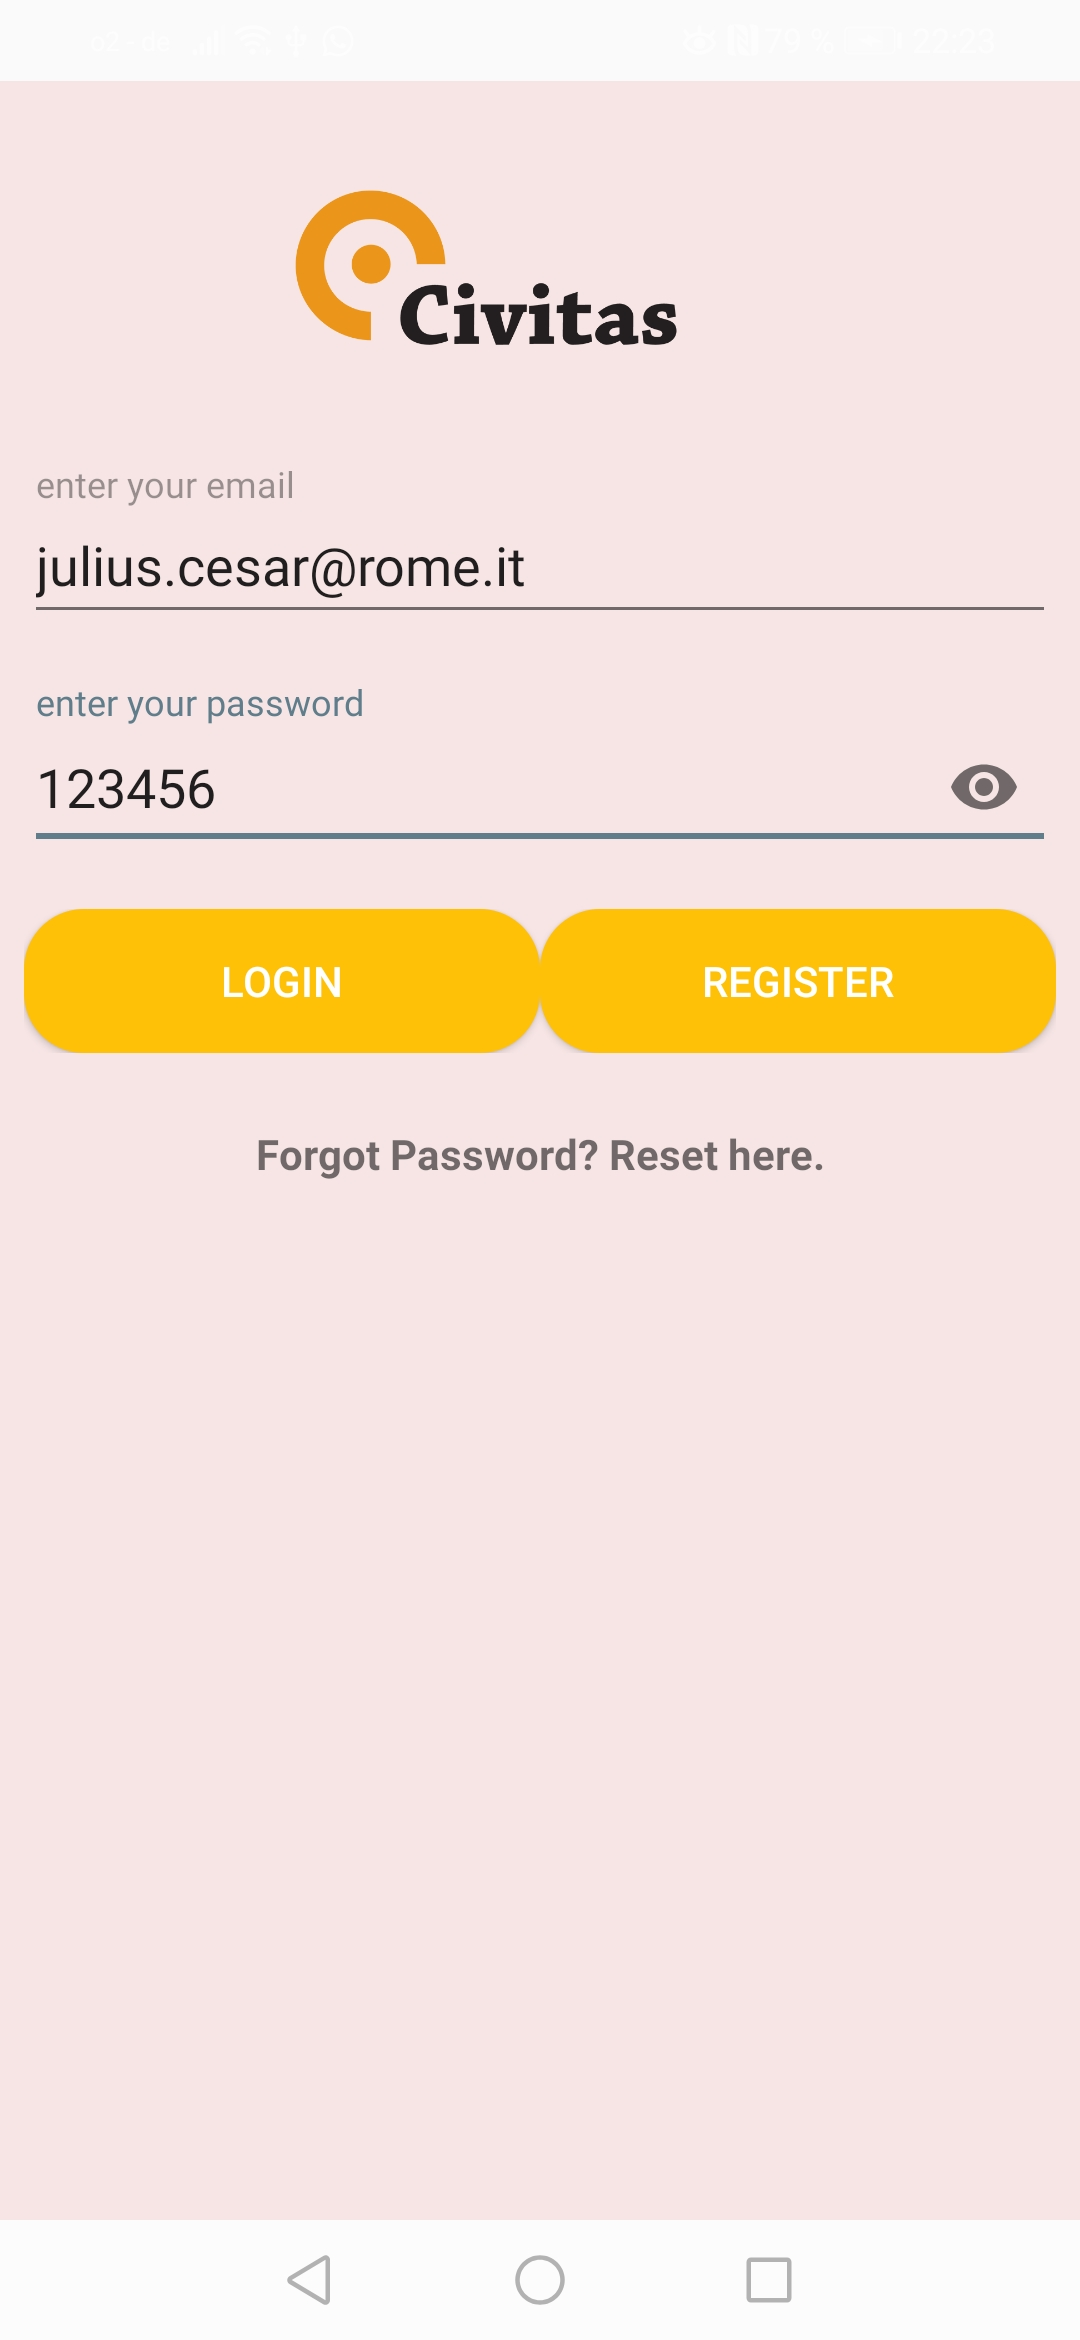
\includegraphics[width=\linewidth]{realization/realization_clear_pw.jpg}
  \caption{Clear password text}
  \label{fig:clear_pw}
\endminipage\hfill
\minipage{0.49\textwidth}
  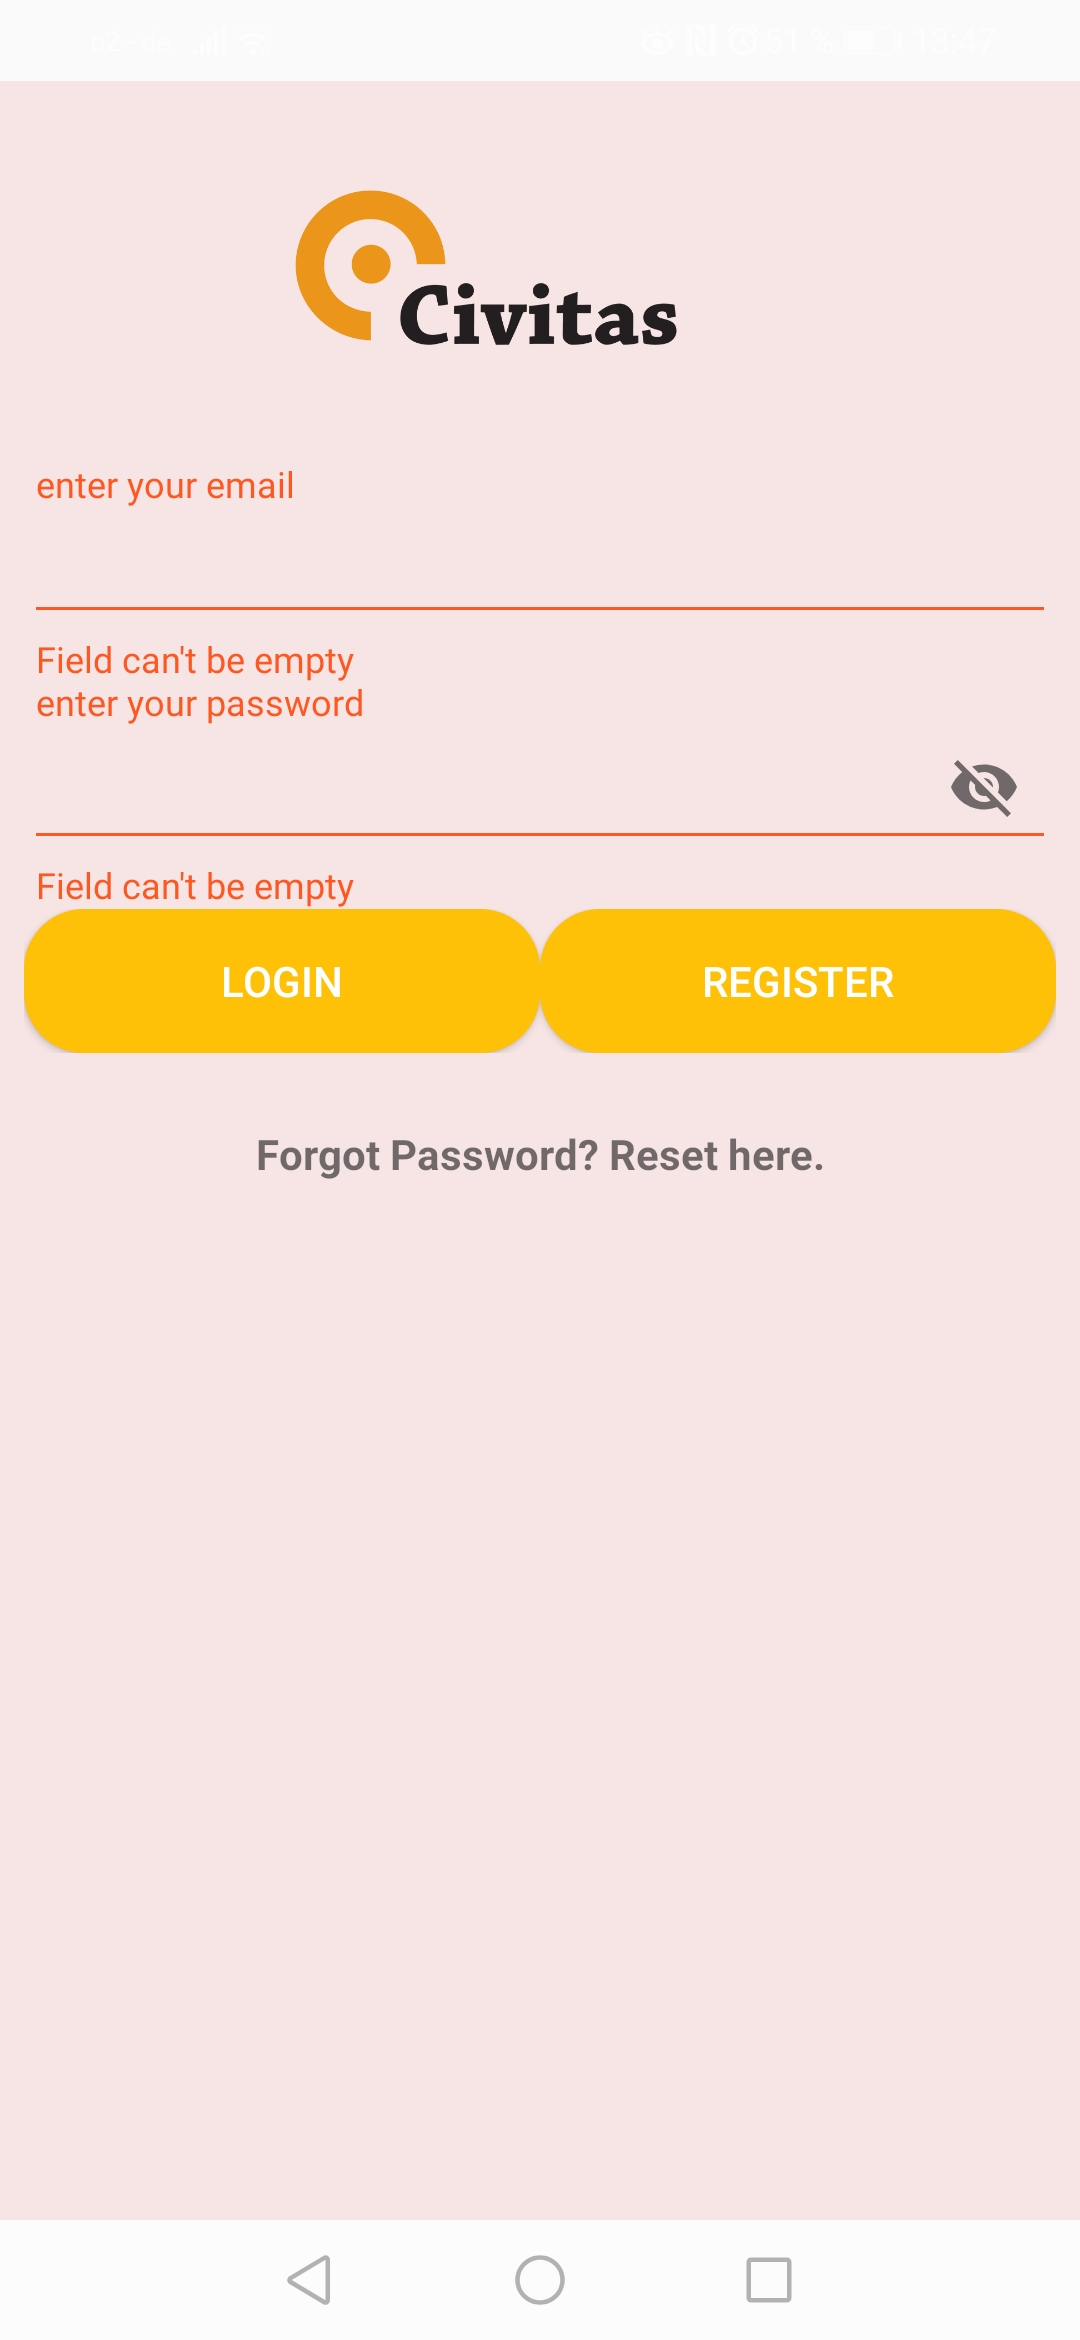
\includegraphics[width=\linewidth]{realization/realization_login_empty_fields.png}
  \caption{Login empty field hints}
  \label{fig:login_empty_fields}
\endminipage\hfill
\caption{Password management}
\label{fig:hint_management}
\end{figure}


\section{Map}
Once a user is logged in, he will enter the map where all existing artefacts are hosted. The map offers the user various possibilities. The usage of them is realized with the GUI elements in the following table (\ref{table:map_gui_elements}).  

\begin{table}[h]
\centering
\begin{tabular}{|l|l|l|}
\hline
\textbf{Index} & \textbf{GUI Element} & \textbf{Task}                   \\ \hline
1              & FloatingActionButton & Create Artefact                 \\ \hline
2              & ActionBar item       & Focus screen on device location \\ \hline
3              & ActionBar item       & Filter/Search artefact          \\ \hline
4              & Navigation drawer    & Navigate through app            \\ \hline
5              & Marker               & Open info window                \\ \hline
6              & InfoWindow           & Provide brief artefact info     \\ \hline
\end{tabular}
\caption{Map GUI elements}
\label{table:map_gui_elements}
\end{table}



One can create an artefact by tapping the \textbf{NewArtefactButton} (1) in the bottom right corner; the resulting artefact will have the coordinates of the device location. However, there is another way to create an artefact as long as the map is visible without a corresponding GUI element. Performing a long click at any place of the map will lead to the NewArtefactFragment as well. An artefact created this way will be connected to the coordinates where the long click was done.

The MyLocation button (2) puts the focus of the screen on the Device location.

The Filter button (3) unfolds the filter menu, where specific parameters can be set. Due to the overlap with the filter menu in the ArtefactListFragment, it will be discussed in its own section.

The Navigation drawer (4) slides in from the left side if a user taps on the Menu icon in the top left corner. From here, one can navigate through the app. Likewise, to the filter menu, it is also available in the ArtefactActivity. Therefore it will also be discussed in its own section.

It remains the marker (5) to be introduced. A Marker is pinned to a particular position on the Map and can carry information about nearly every topic one can imagine. In this case, it represents an artefact. A click on a Marker will open an info window (6) with the name and the description of the artefact. Another click on the InfoWindow leads the user to the ArtefactDetailFragment.

An impression of the map delivers image set (fig. \ref{fig:civitas_map}).

\begin{figure}[!htb]
\minipage{0.49\textwidth}
  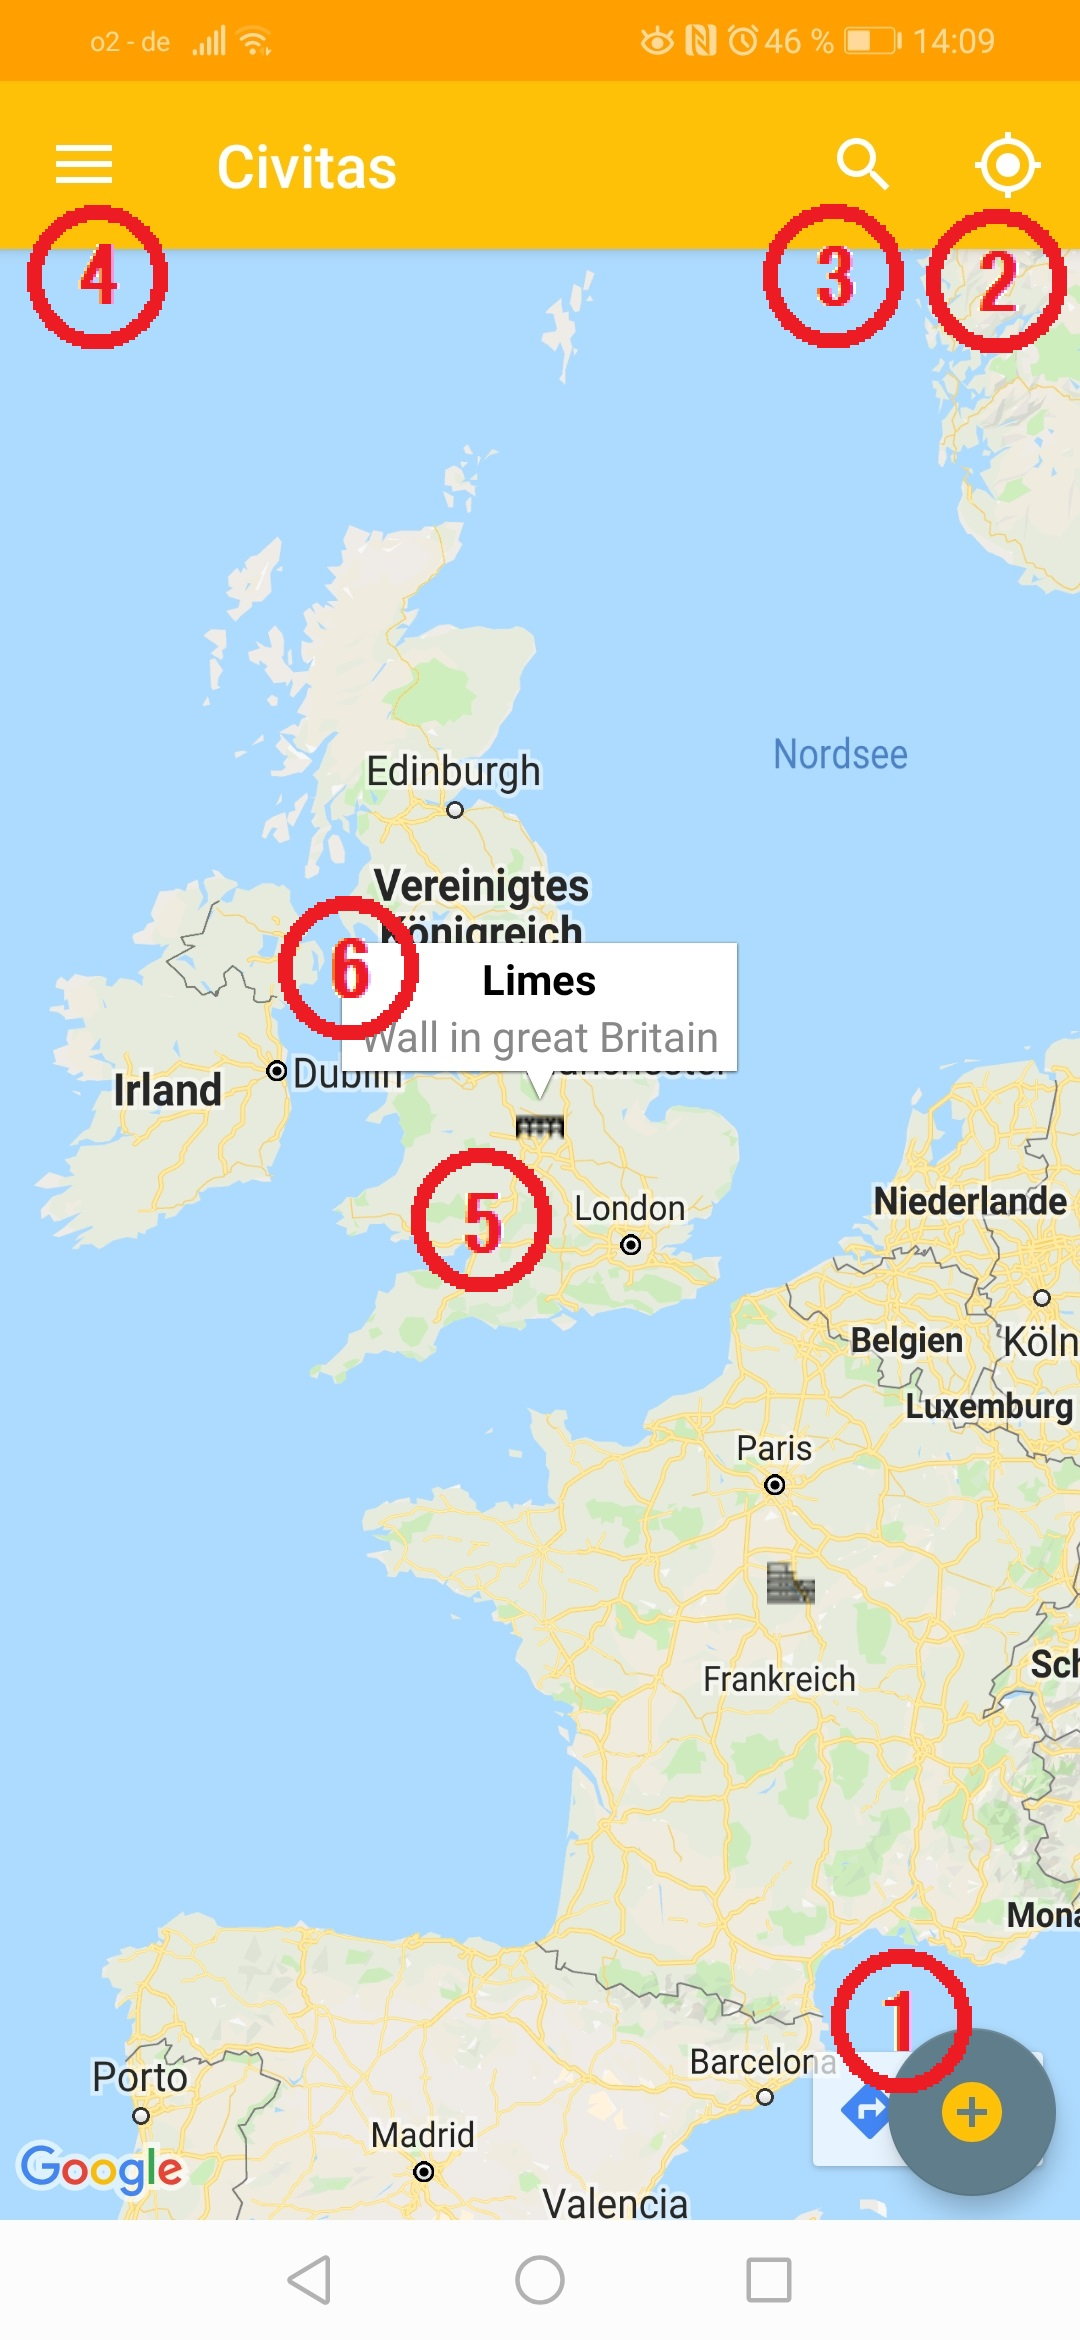
\includegraphics[width=\linewidth]{realization/realization_map_with_info_window.png}
  \caption{Map with marker info window opened}
  \label{fig:map_info_window}
\endminipage\hfill
\minipage{0.49\textwidth}
  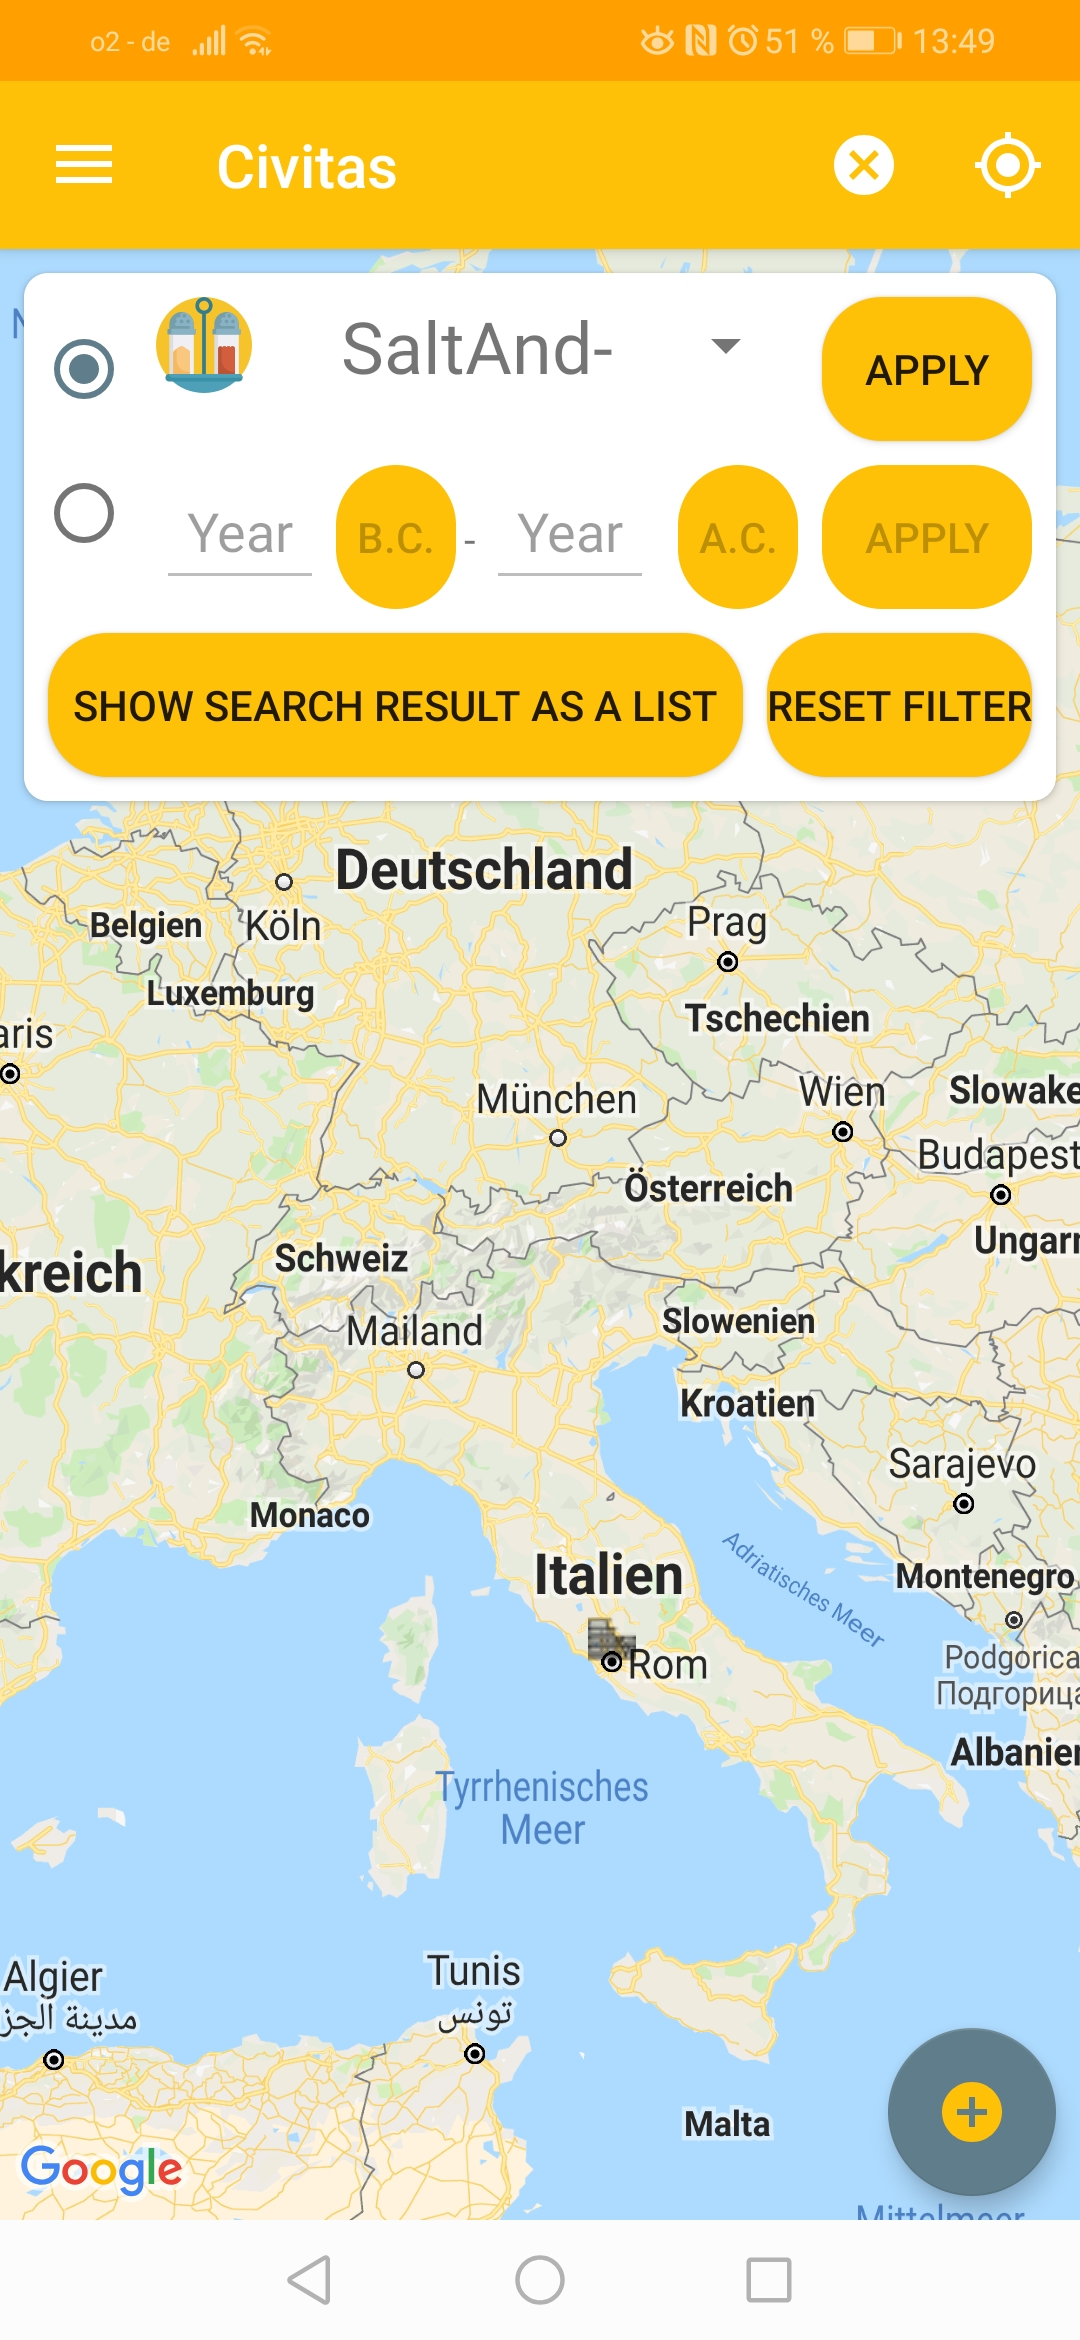
\includegraphics[width=\linewidth]{realization/realization_map_filter.png}
  \caption{Map with unfolded filter menu}
  \label{fig:map_filter}
\endminipage\hfill
\caption{Civitas map}
\label{fig:civitas_map}
\end{figure}


\section{Artefact Management}
The most common way of leaving the map leads to an artefact related destination. The \textbf{ArtefactActivity} is the host of the \textbf{NewArtefactFragment}, \textbf{EditArtefactFragment}, ArtefactDetailFragment, and the \textbf{ArtefactListFragment}. These Fragments determine artefact management by providing GUI elements for the current purpose. The GUI elements are connected to Android API components to provide the required information for each purpose. The ArtefactActivity provides the following GUI elements to its Fragments: \textbf{Navigation Drawer} and \textbf{ActionBar} items. Hence, one can access the Navigation Drawer everywhere within artefacts related events. Depending on the currently logged in user the ActionBar items changes. Due to its user rights, editing or deleting icons are visible or not.

\subsection{Create Artefact}
An artefact is a set of information about a historical monument. The \textbf{NewArtefactFragment} contains the following GUI elements: CardView, ImageView, EditText, ImageButton, and Spinner. 
One can choose whether to take a picture with the camera or from the gallery. Furthermore, metadata is required, such as name, description, age, and category. There is a part of an audio record too, but unfortunately, this feature is not implemented due to a lack of time.
The following image set displays the create artefact process (fig. \ref{fig:create_artefact}).


\begin{figure}[htb]

\minipage{0.30\textwidth}
  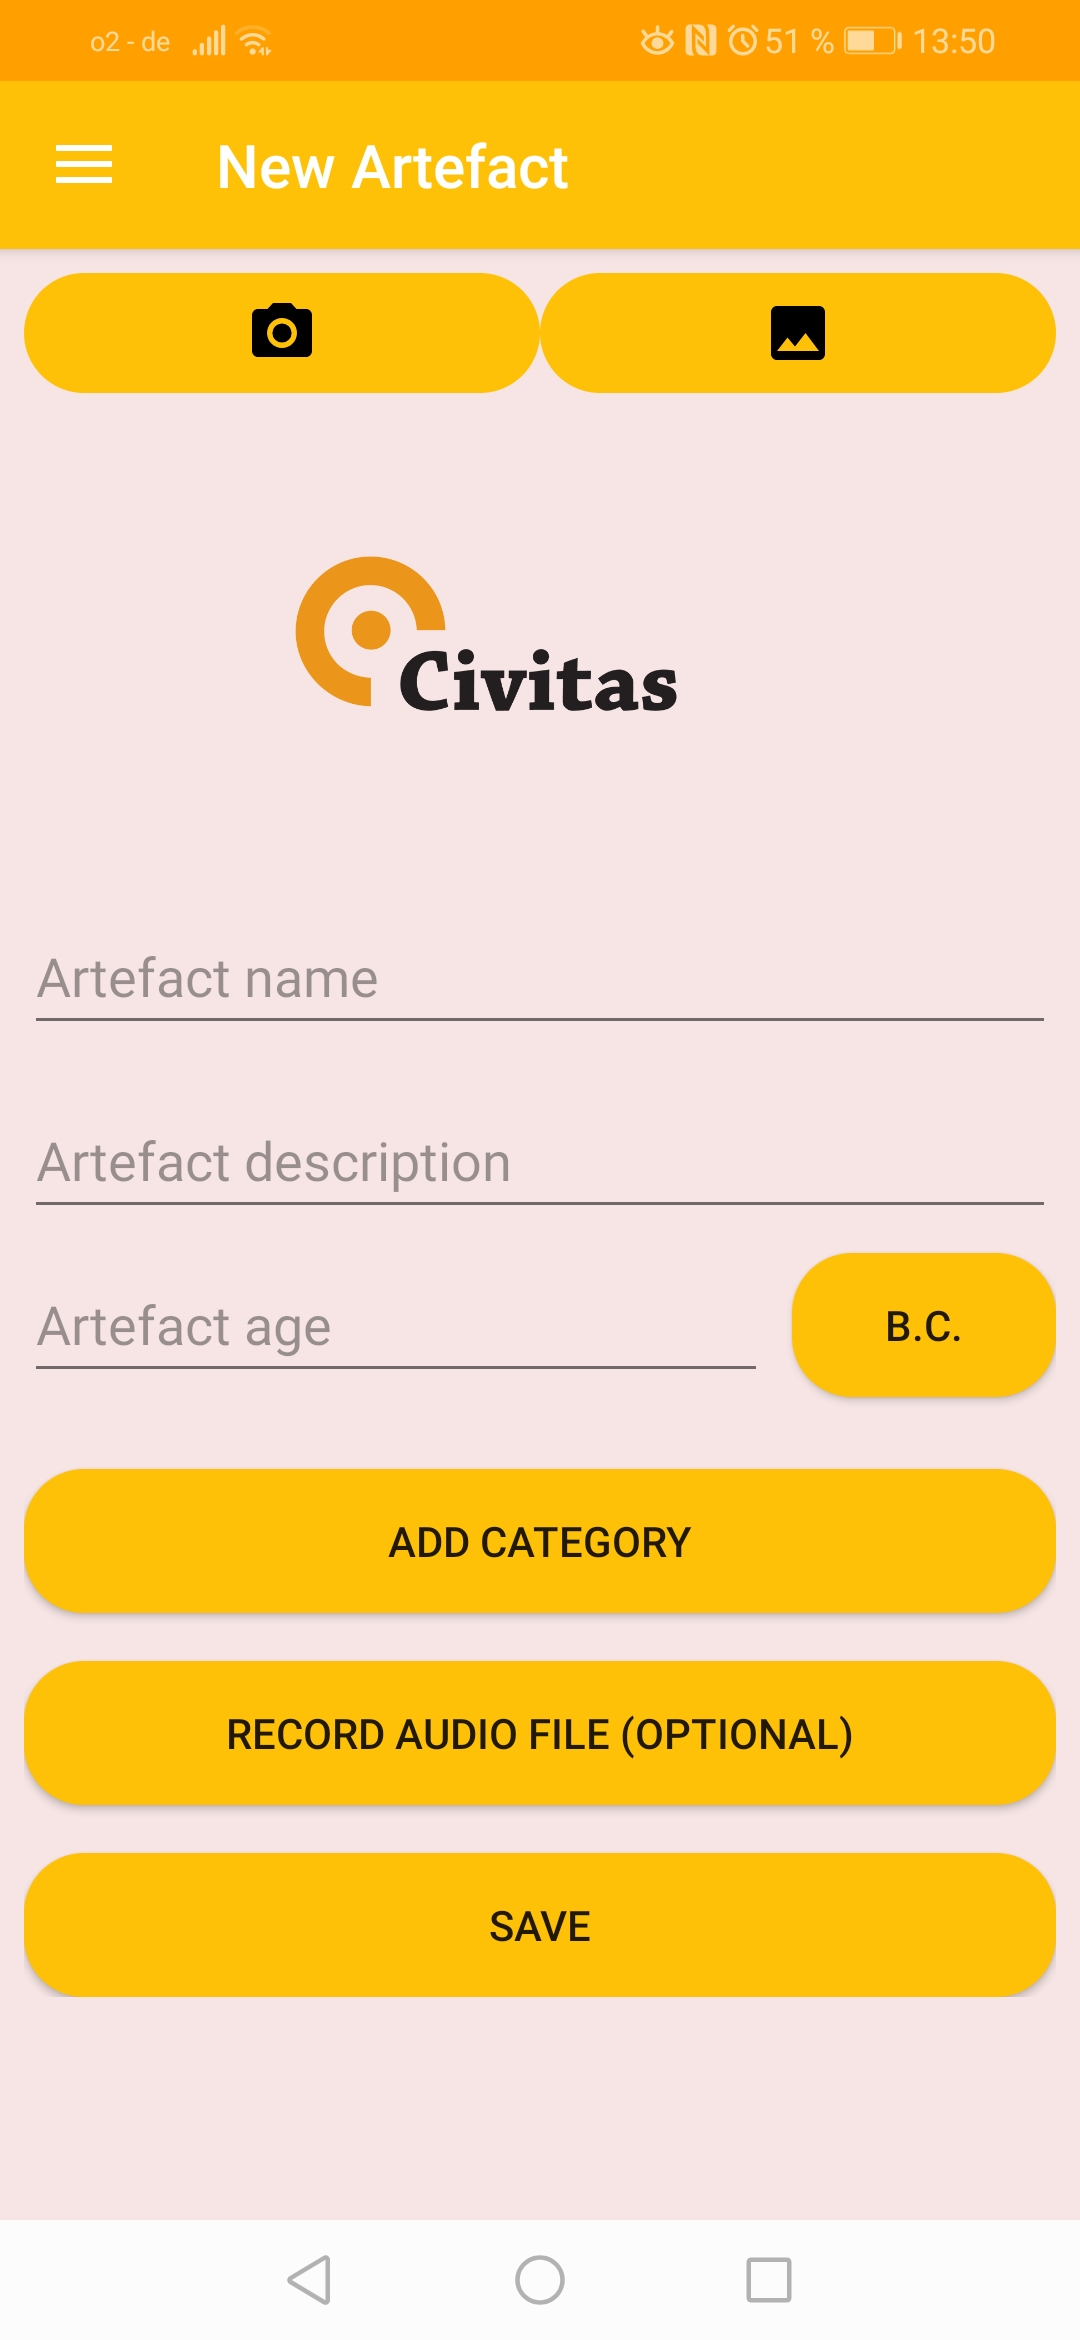
\includegraphics[width=\linewidth]{realization/realization_new_artefact.png}
  \caption{New artefact    fragment}\label{fig:realization_new_artefact}
\endminipage\hfill
\minipage{0.30\textwidth}
  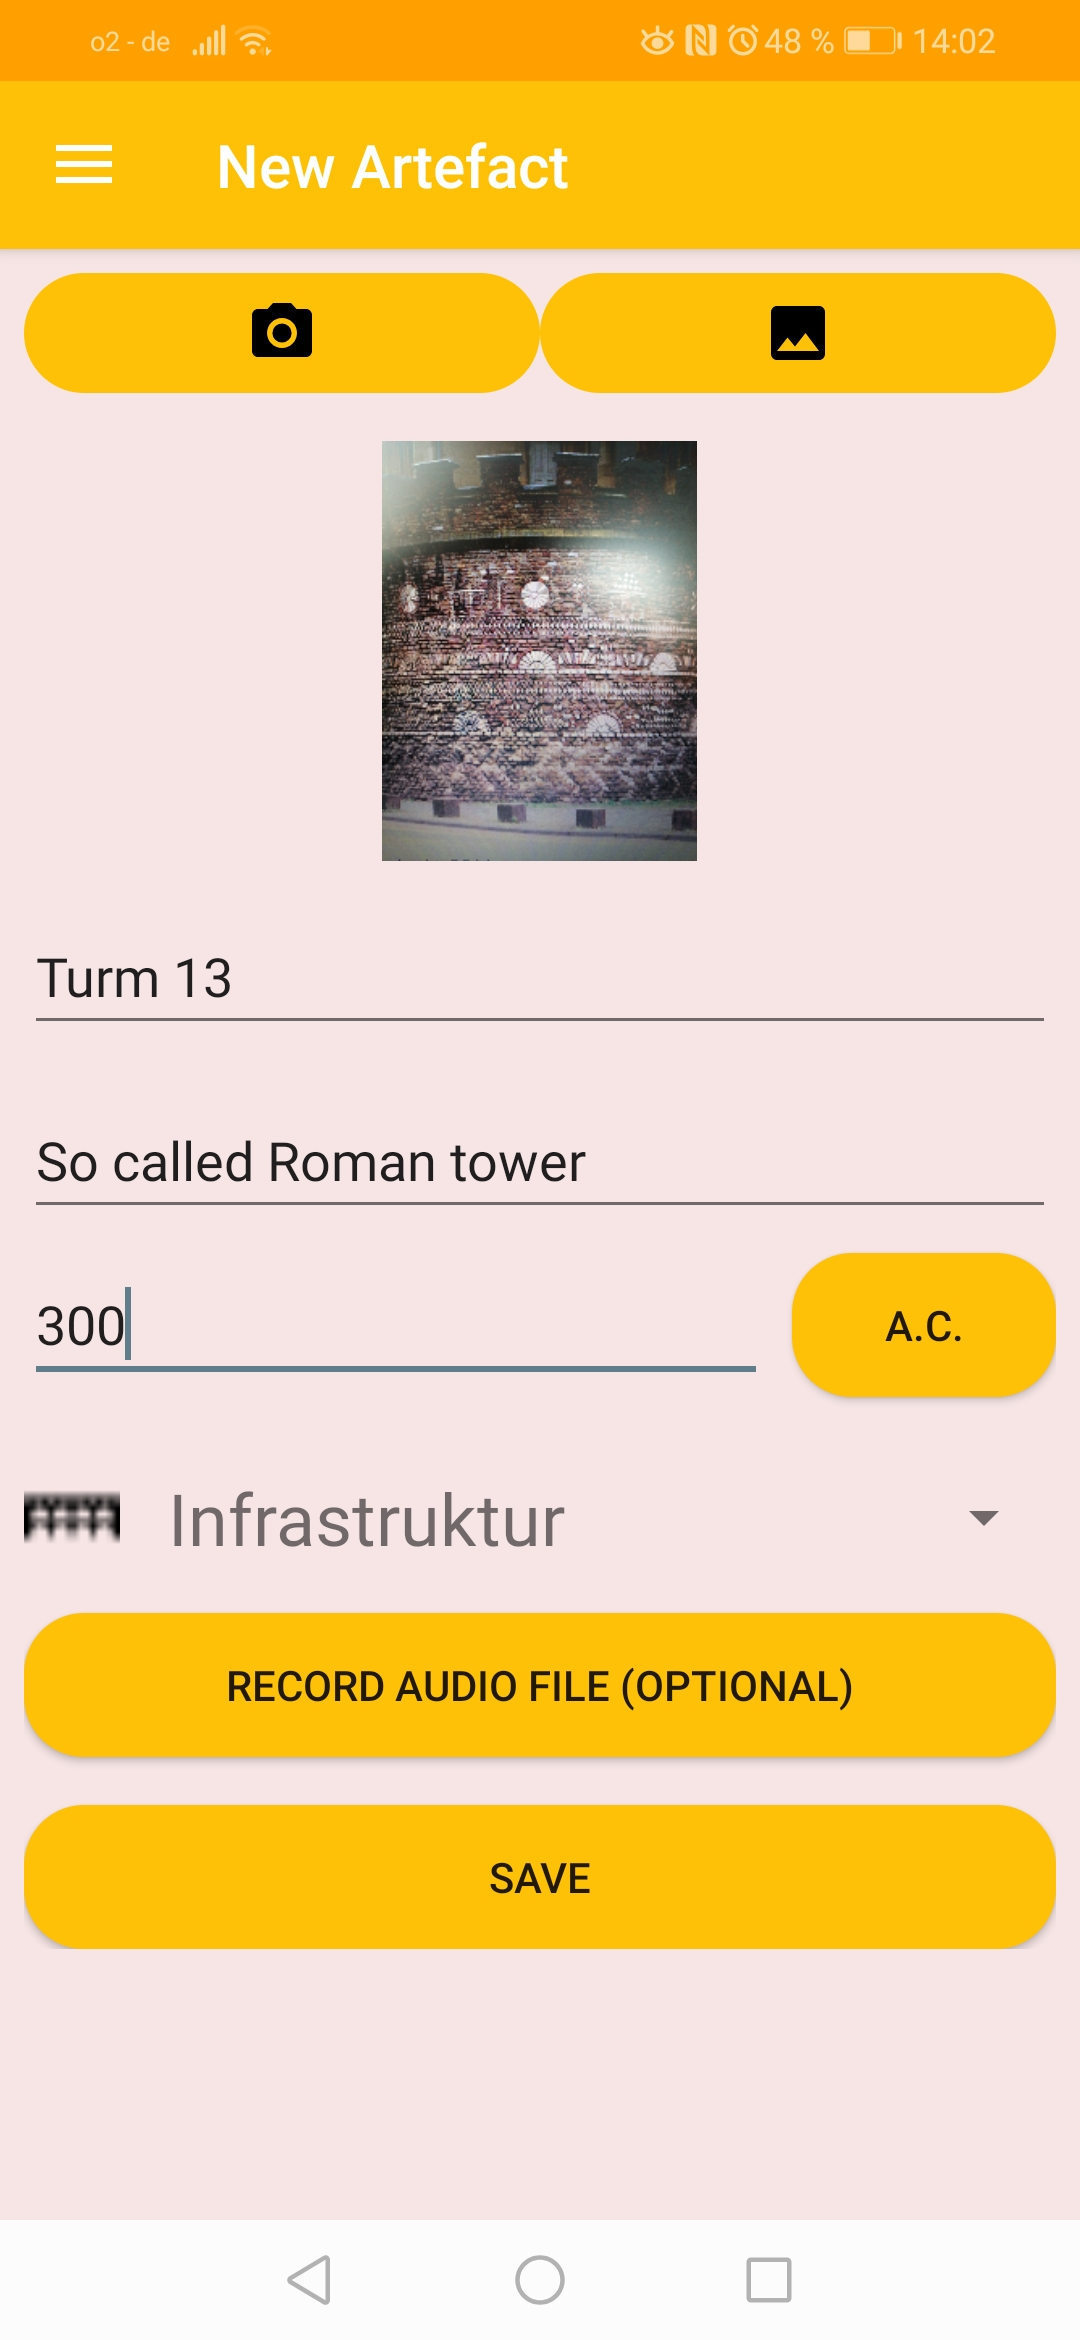
\includegraphics[width=\linewidth]{realization/realization_new_artefact_with_input.png}
  \caption{Artefact with input}\label{fig:realization_new_artefact_with_input}
\endminipage\hfill
\minipage{0.30\textwidth}
  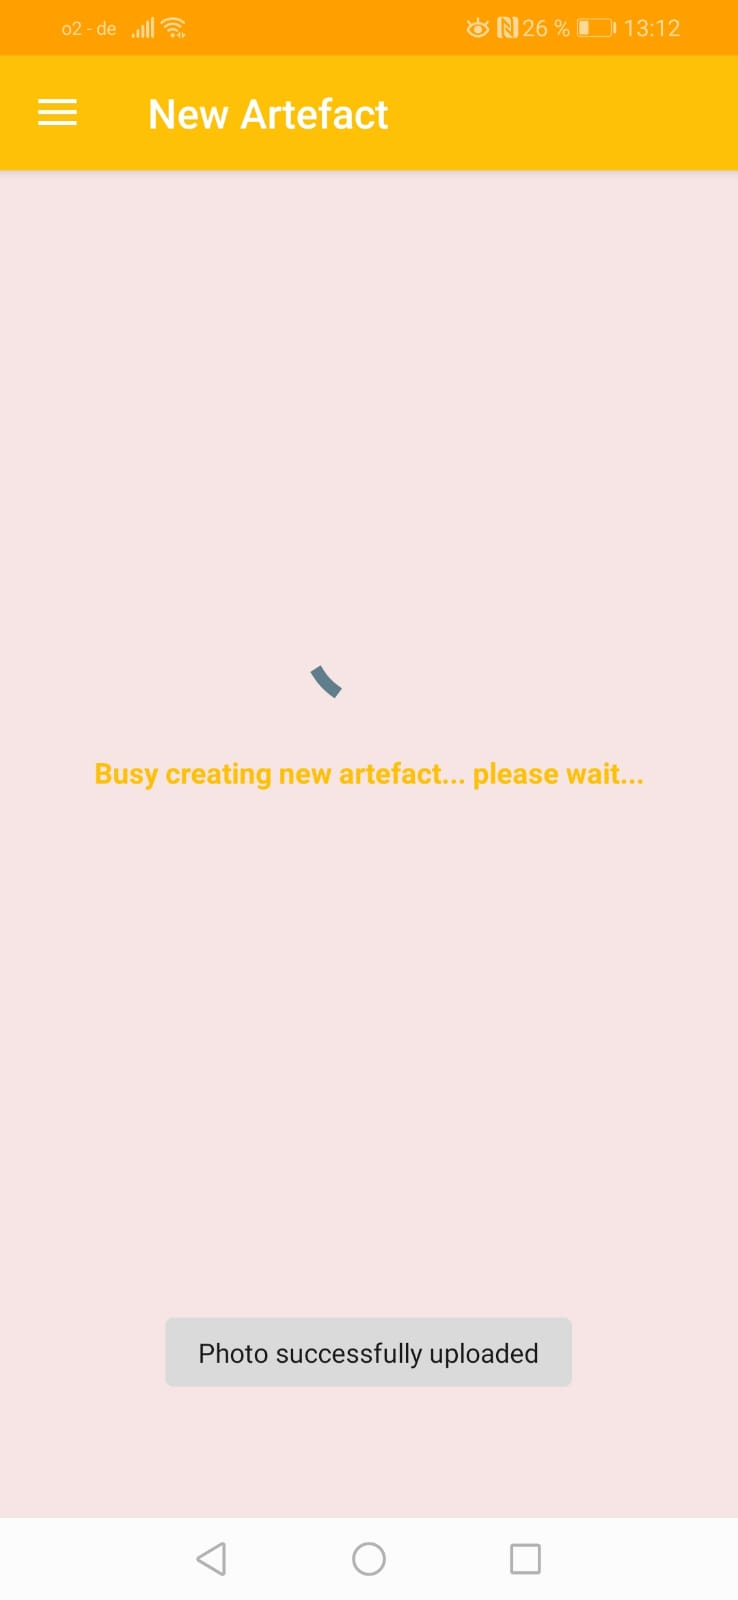
\includegraphics[width=\linewidth]{realization/realization_new_artefact_info.png}
  \caption{Progress information}\label{fig:realization_new_artefact_info}
\endminipage\hfill
\caption{Create new artefact}
\label{fig:create_artefact}
\end{figure}


Once the user has created an artefact, he is the owner of it, and the \textbf{ArtefactDetailFragment} and the \textbf{ArtefactListFragment} are accessable.

\newpage
\subsection{Artefact List}
This part of the app can be reached via the navigation drawer. It contains the following GUI elements: RecyclerView, CardView, ImageView, and TextView.

The RecyclerView is responsible for listing the artefact items. The items are build from the mentioned GUI elements. They provide brief information about the artefacts. Tap an artefact item leads to the ArtefactDetailFragment for further information.

\begin{figure}[H]
\centering
\minipage{0.49\textwidth}
  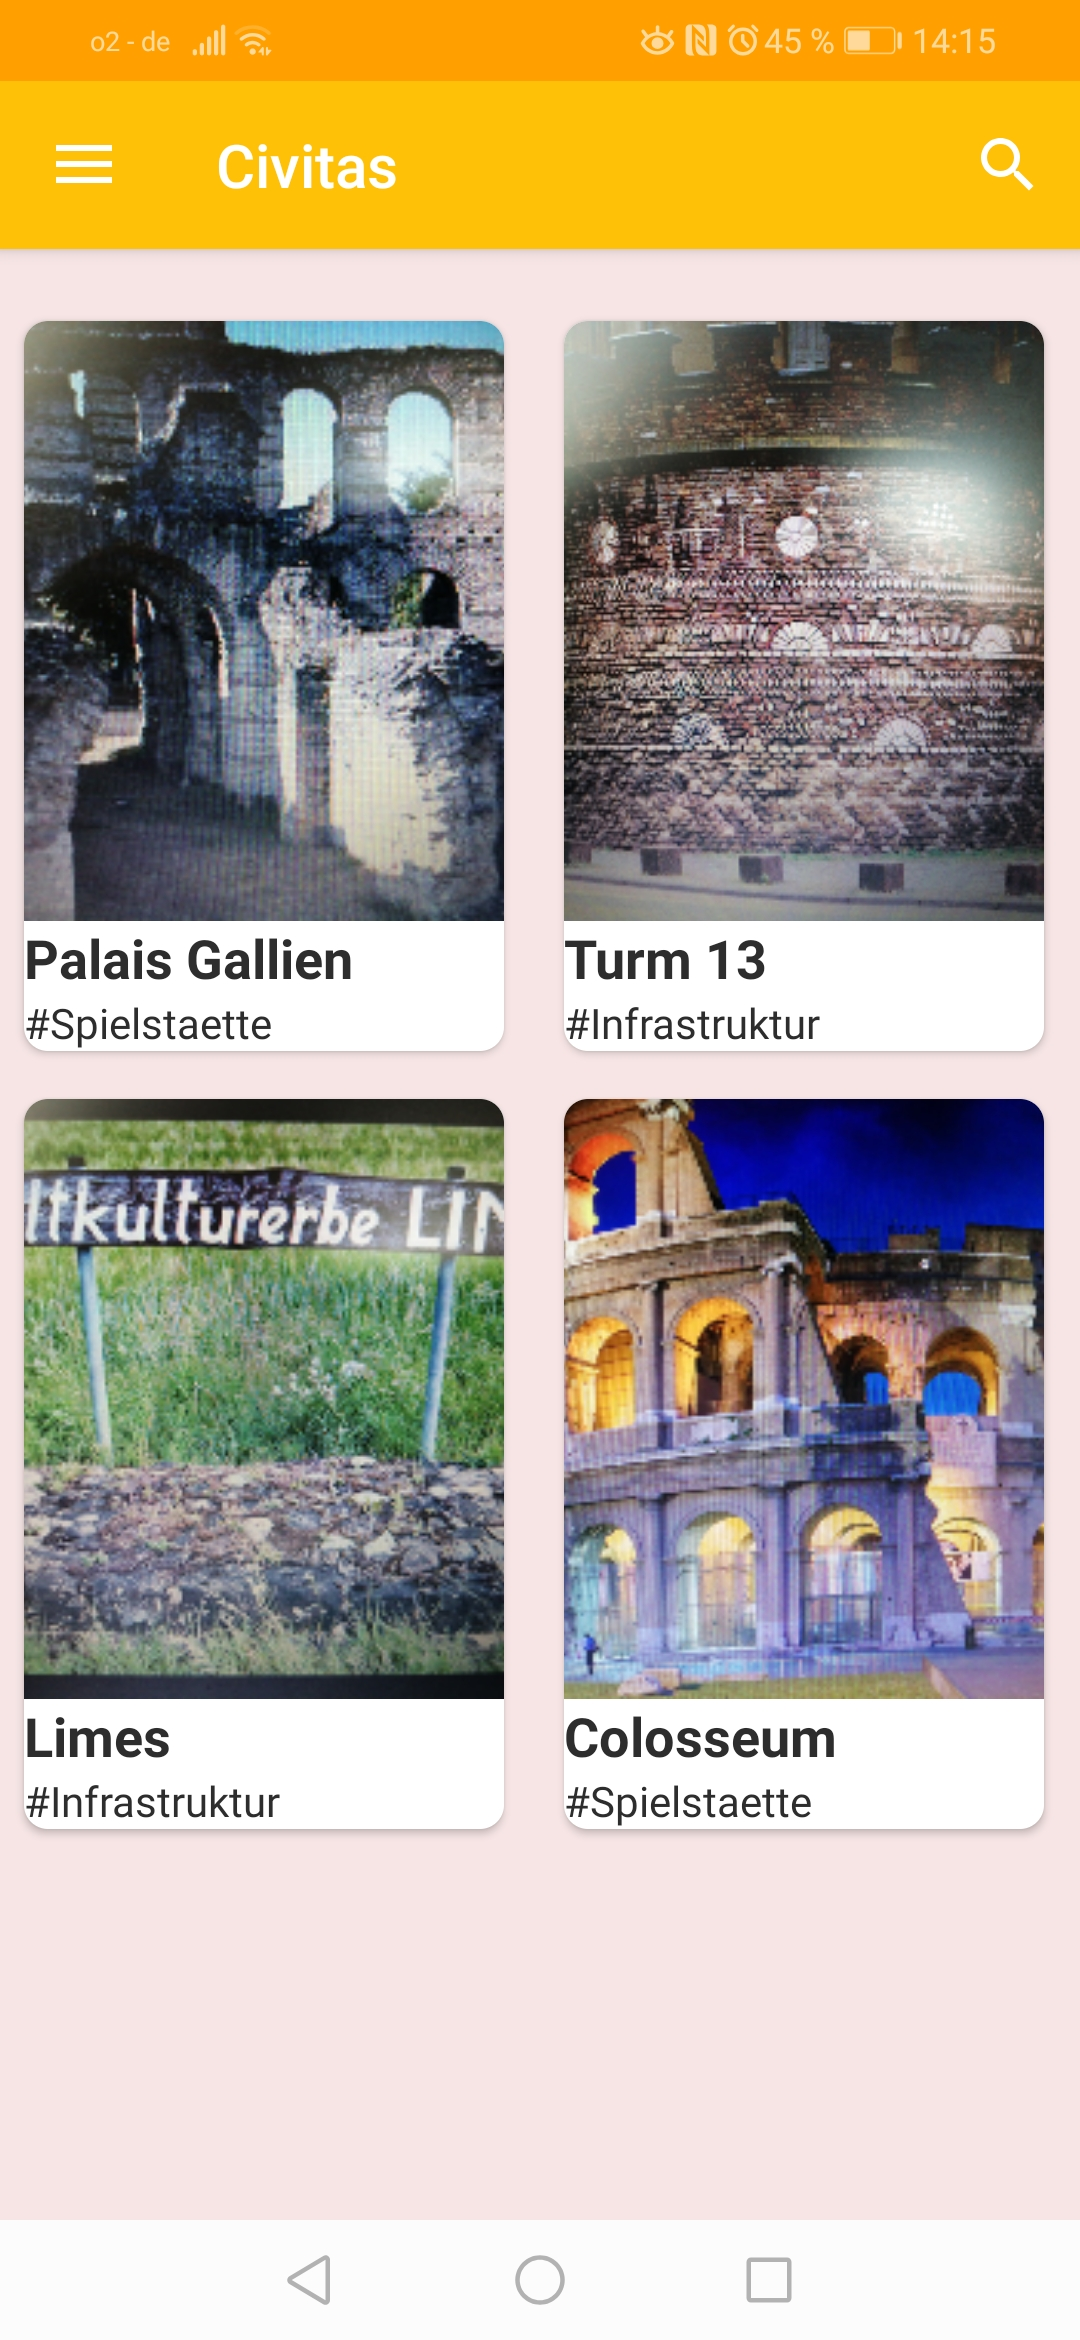
\includegraphics[width=\linewidth]{realization/realization_list.png}
  \caption[ArtefactListFragment]{ArtefactListFragment}
  \label{fig:realization_list}
\endminipage\hfill
\end{figure}

One can tap on the magnifying glass to unfold the filter menu. As mentioned before the filter menu will be explained in its own section.

\subsection{Artefact Detail}
To provide content, the ArtefactDetailFragment use this GUI elements: CardView, ImageView, TextView, ActionBar items. 
Depending on if the user is also the owner of the artefact, the ActionBar items for editing and deleting become visible. One can return to the artefact on the map by taping the crosshair icon within the ActionBar. This icon is always visible. Image set (fig. \ref{fig:artefact_detail}) displays the two states, a) user is artefact owner, or b) not.

\begin{figure}[htb]
\minipage{0.49\textwidth}
  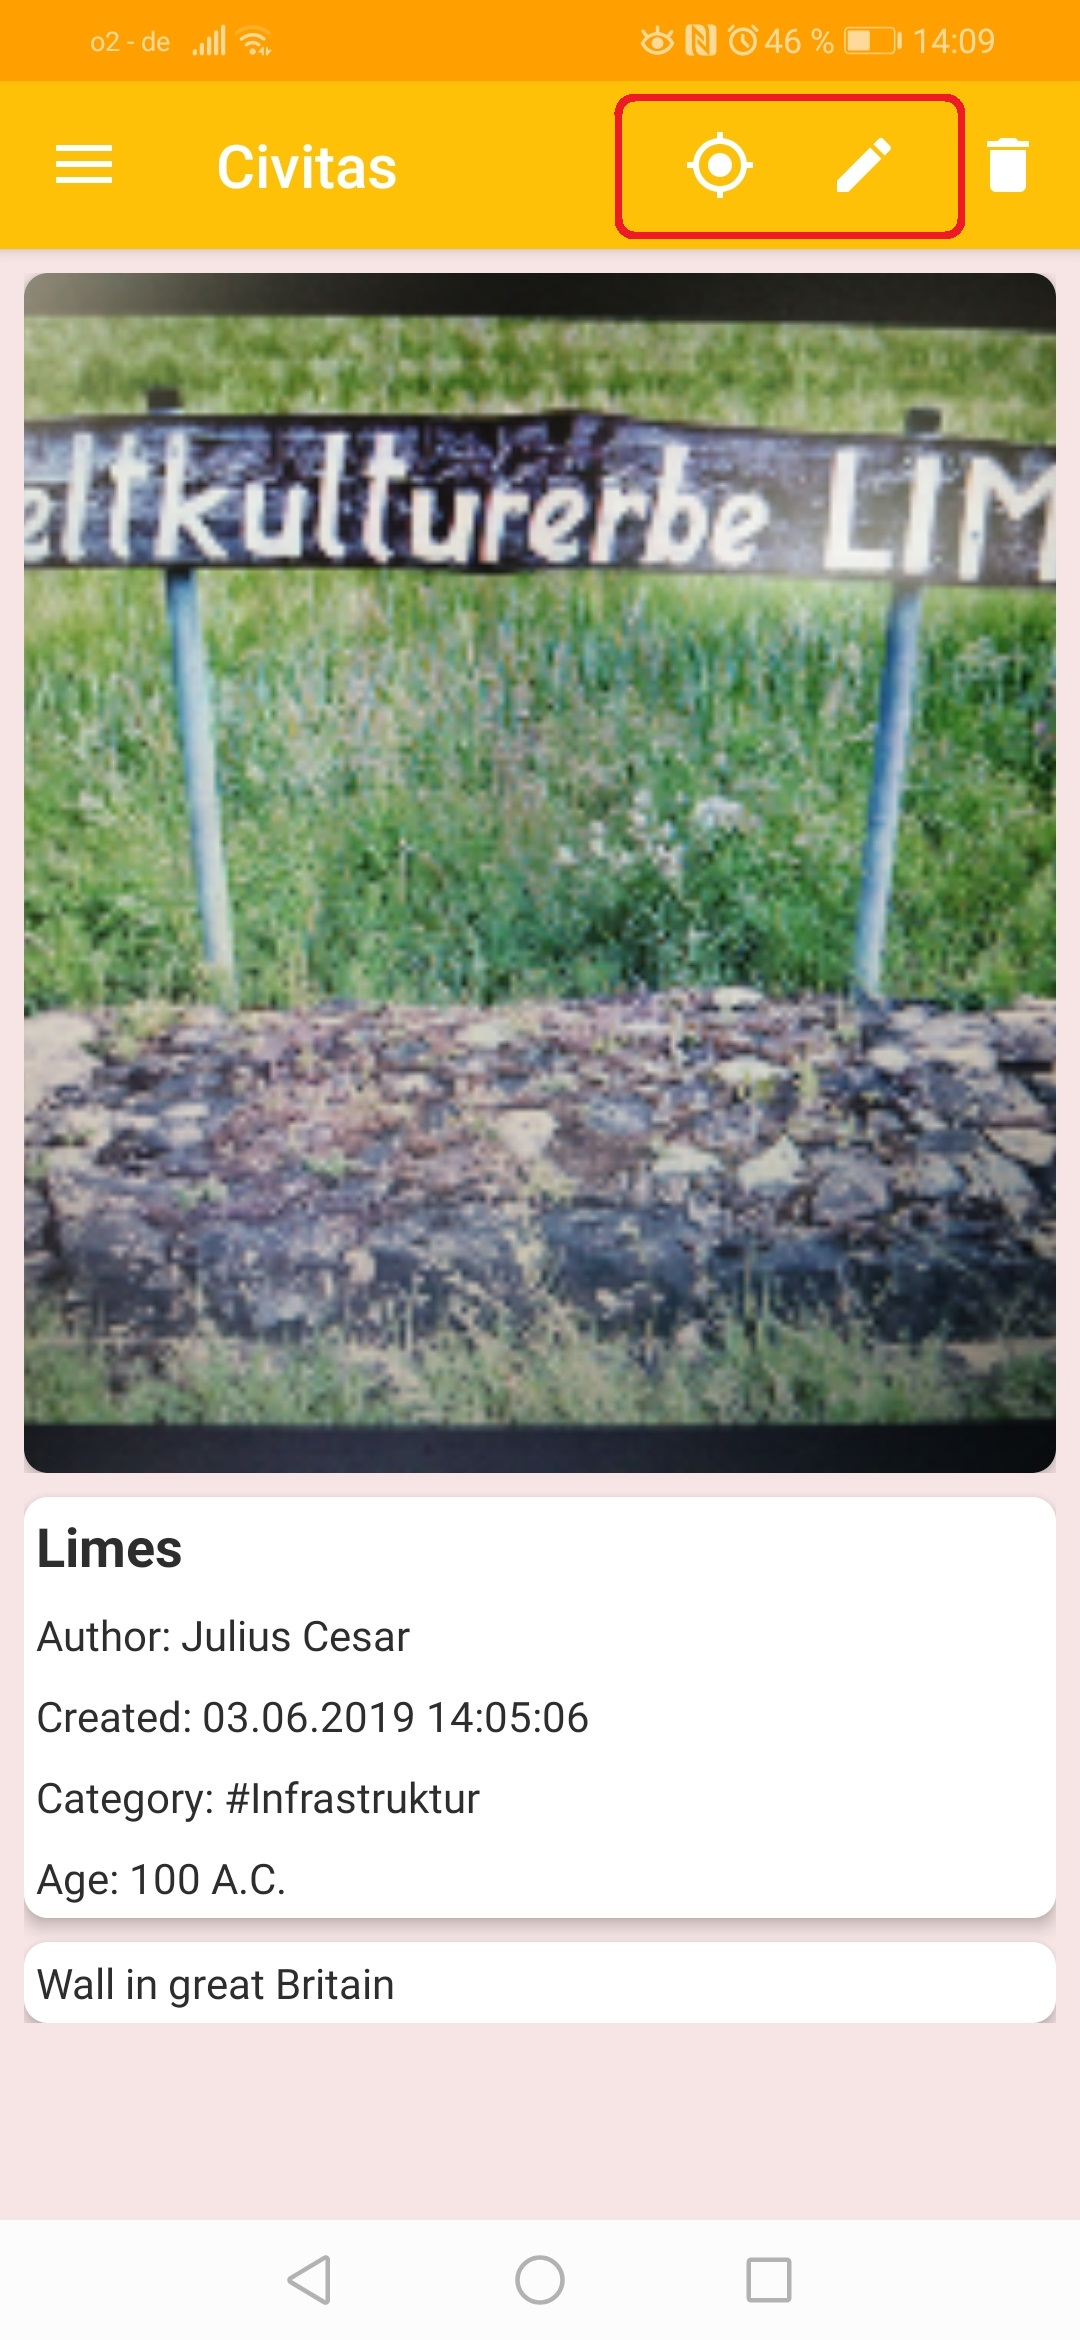
\includegraphics[width=\linewidth]{realization/realization_artefact_detail_owner.png}
  \caption{User is artefact owner}\label{fig:realization_artefact_detail_owner}
\endminipage\hfill
\minipage{0.49\textwidth}
  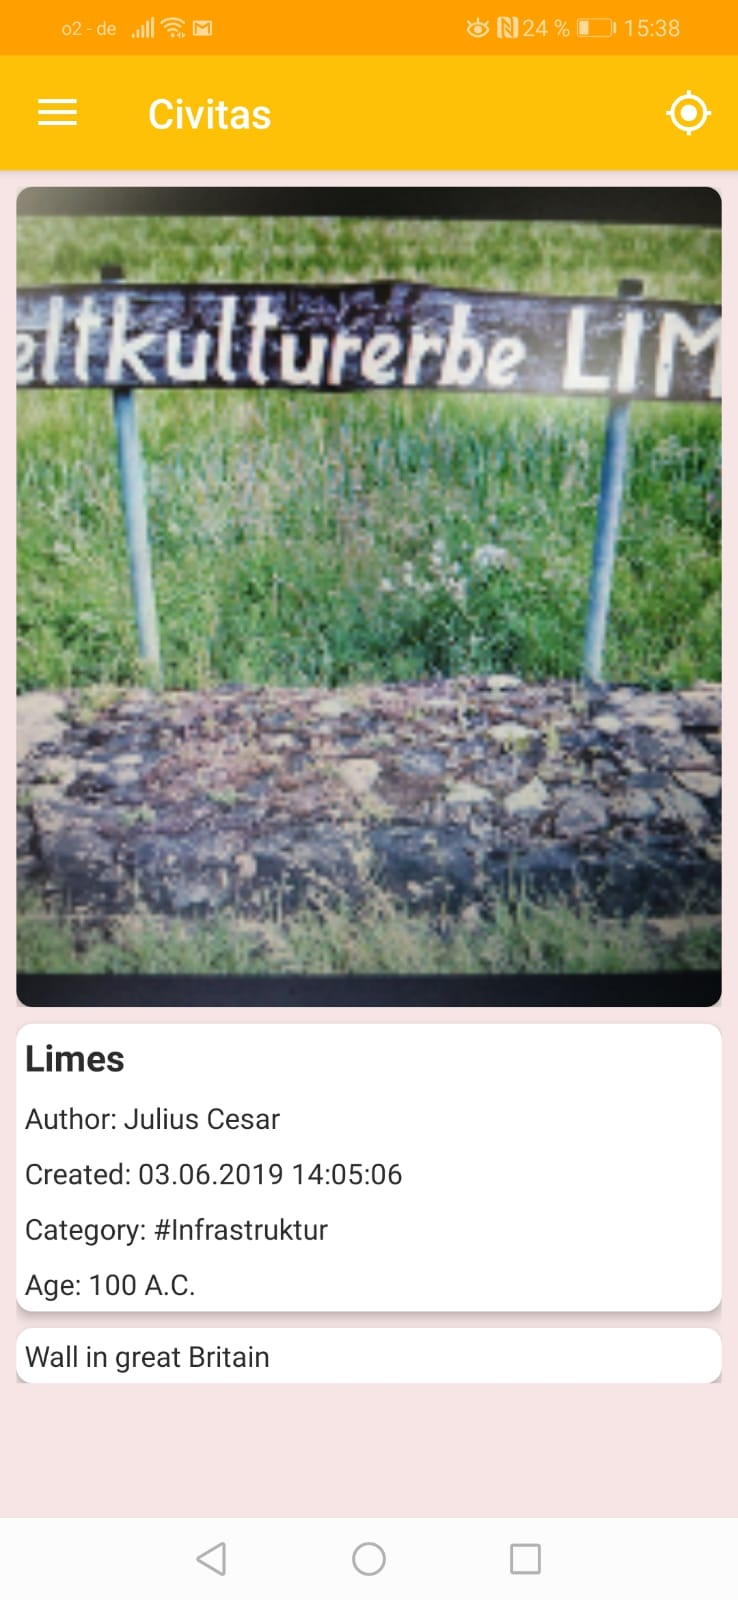
\includegraphics[width=\linewidth]{realization/realization_artefact_detail.png}
  \caption{User is not artefact owner}\label{fig:realization_artefact_detail}
\endminipage\hfill
\caption{Artefact detail}
\label{fig:artefact_detail}
\end{figure}

\subsection{Edit/Delete Artefact}
Editing or deleting artefacts can have a huge impact on the Civitas database. In order to avoid abuse of the stored artefact data, one can edit or delete artefacts only if one is the owner. Since the delete process erases an artefact, it has no other realization pattern than the trash can icon within the ArtefactDetailFragment. An alert dialog gets displayed to ensure the user wants to delete the artefact (fig. \ref{fig:realization_delete_dialog}). Once the process is started, the user will be kept up to date about the progress status. However, the editing process is more complex, and a click on the pen icon leads to the EditArtefactFragment. During the transition from ArtefactDetailFragment to EditArtefactFragment, one also gets progress information about the loading process. After this process is terminated, the arriving screen looks quite similar to the NewArtefactFragment, with the difference, that all artefact values are set. Now, one can change any value (fig. \ref{fig:realization_edit_artefact}.

\begin{figure}[H]
\centering
\minipage{0.49\textwidth}
  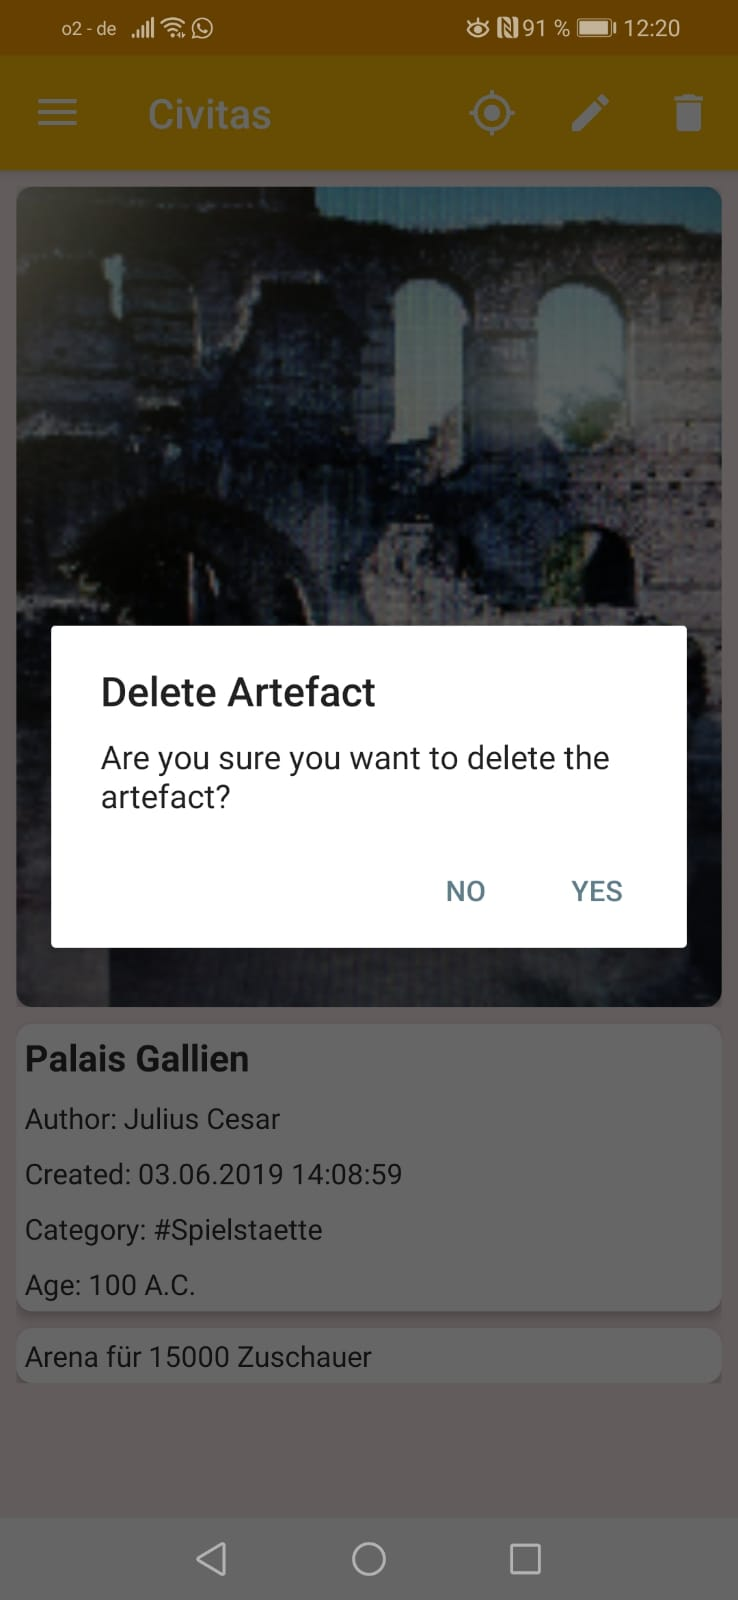
\includegraphics[width=\linewidth]{realization/realization_delete_dialog.png}
  \caption[Delete dialog]{Delete dialog}\label{fig:realization_delete_dialog}
\endminipage\hfill
\minipage{0.49\textwidth}
  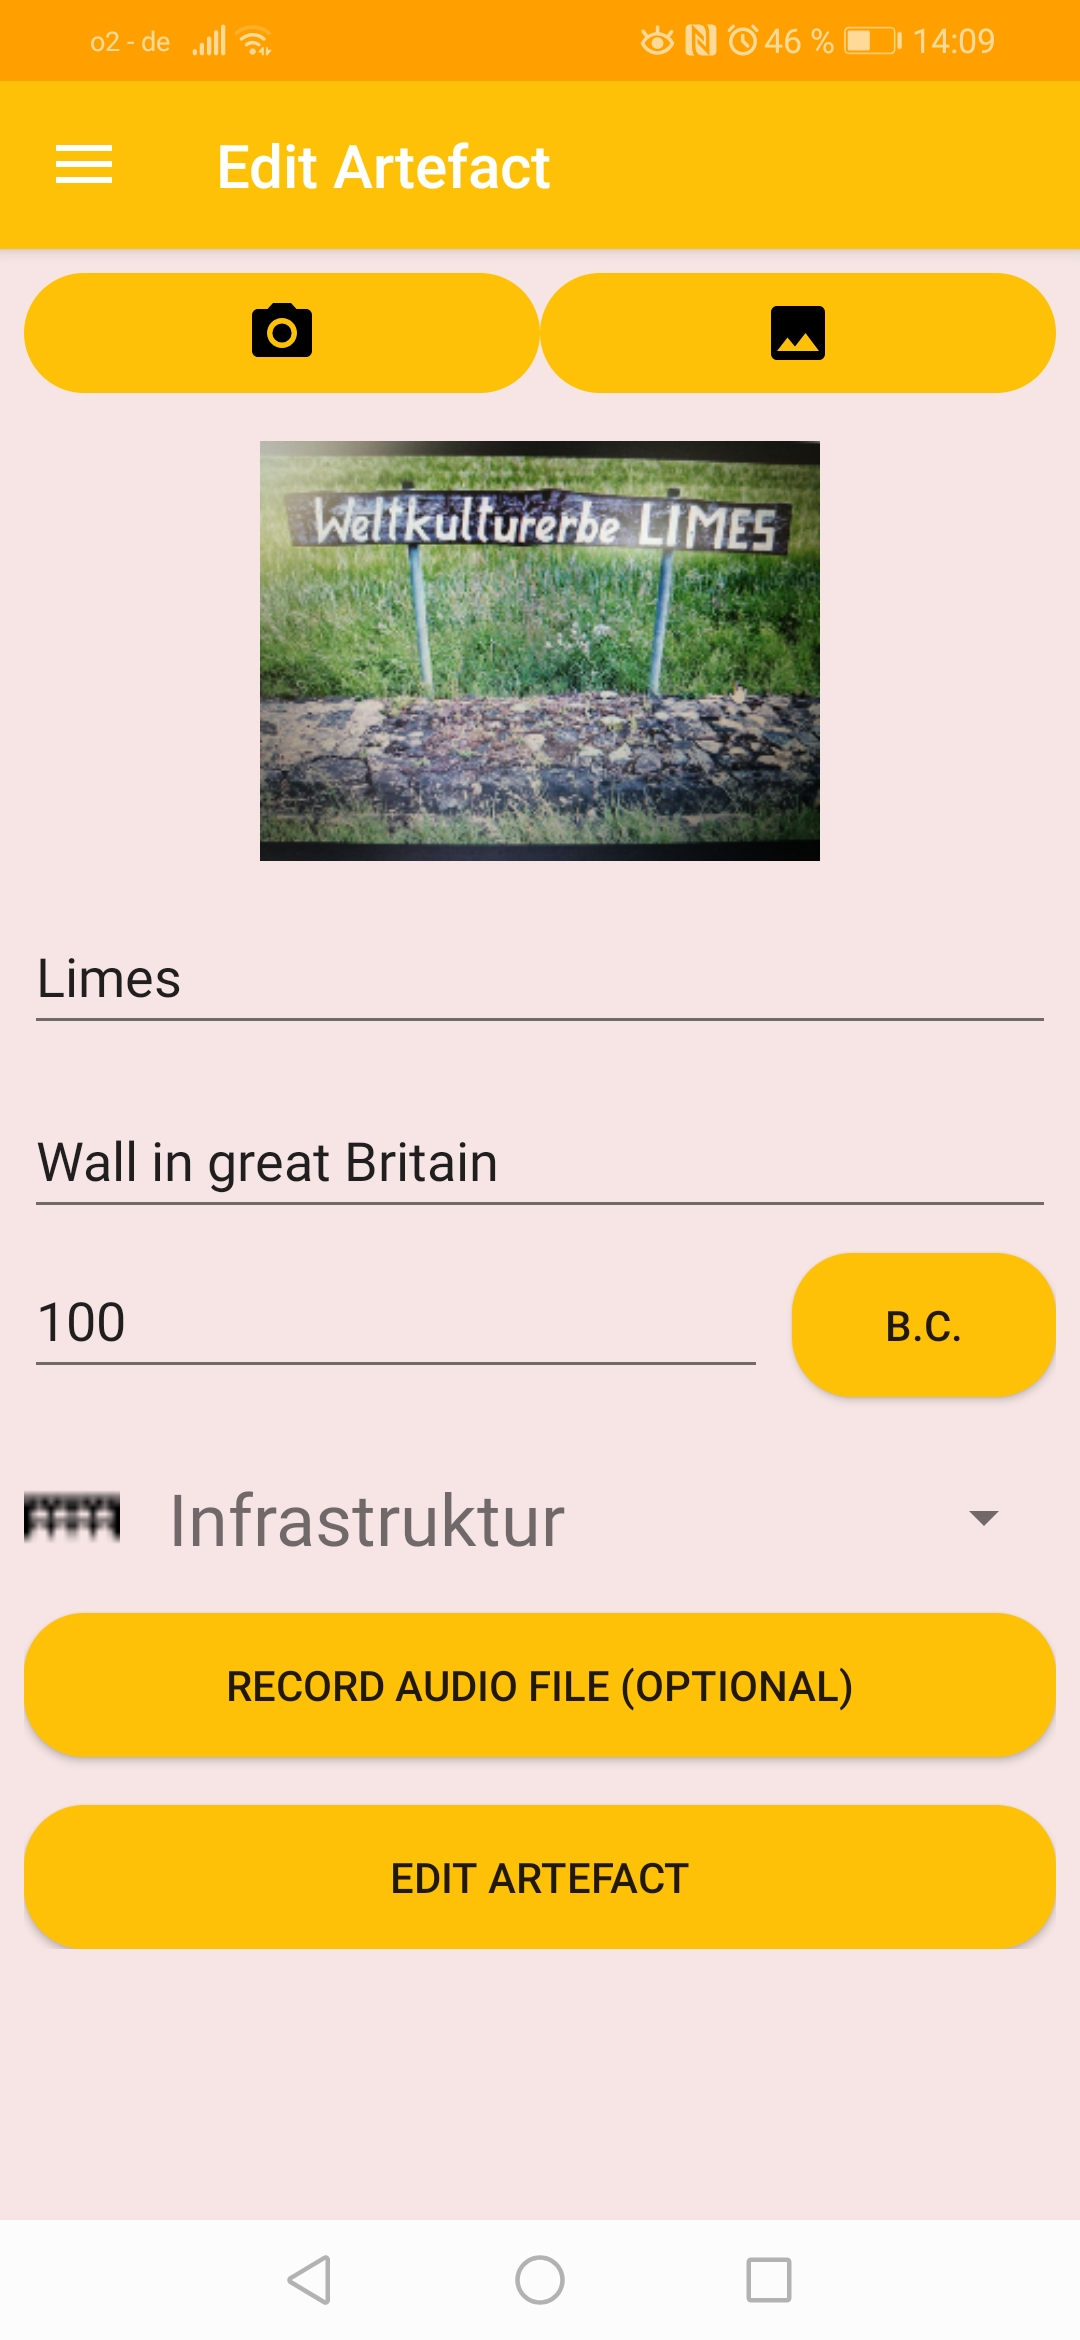
\includegraphics[width=\linewidth]{realization/realization_edit_artefact.png}
  \caption[Editing an artefact]{Editing an artefact}
  \label{fig:realization_edit_artefact}
\endminipage\hfill
\caption{Manipulating artefacts}
\label{fig:artefact_edit_delete}
\end{figure}

\section{Imprint}


The imprint is based in the \textbf{ImpressumActivity} and is realized by a \textbf{WebView}. Accessing the imprint from the Navigation Drawer, one gets redirected to the customer website of the Civitas project (fig. \ref{fig:imprint}).

\begin{figure}[H]
\centering
\minipage{0.49\textwidth}
  
\includegraphics[width=\linewidth]{realization/imprint.png}
  \caption[Imprint]{Imprint}
  \label{fig:imprint}
\endminipage\hfill
\end{figure}

\section{Common}

\subsection{Navigation}
One can explore the Civitas app in various ways. A central GUI element for navigation purpose is the Navigation Drawer. This drawer slides in from the left side, if one performs a swipe gesture from this direction, or tap the menu icon in the top left corner. It is accessible within the MapActivity and the ArtefactActivity. Once the drawer is expanded, one can choose several options (fig. \ref{fig:realization_drawer}).

\begin{figure}[H]
\centering
\minipage{0.49\textwidth}
  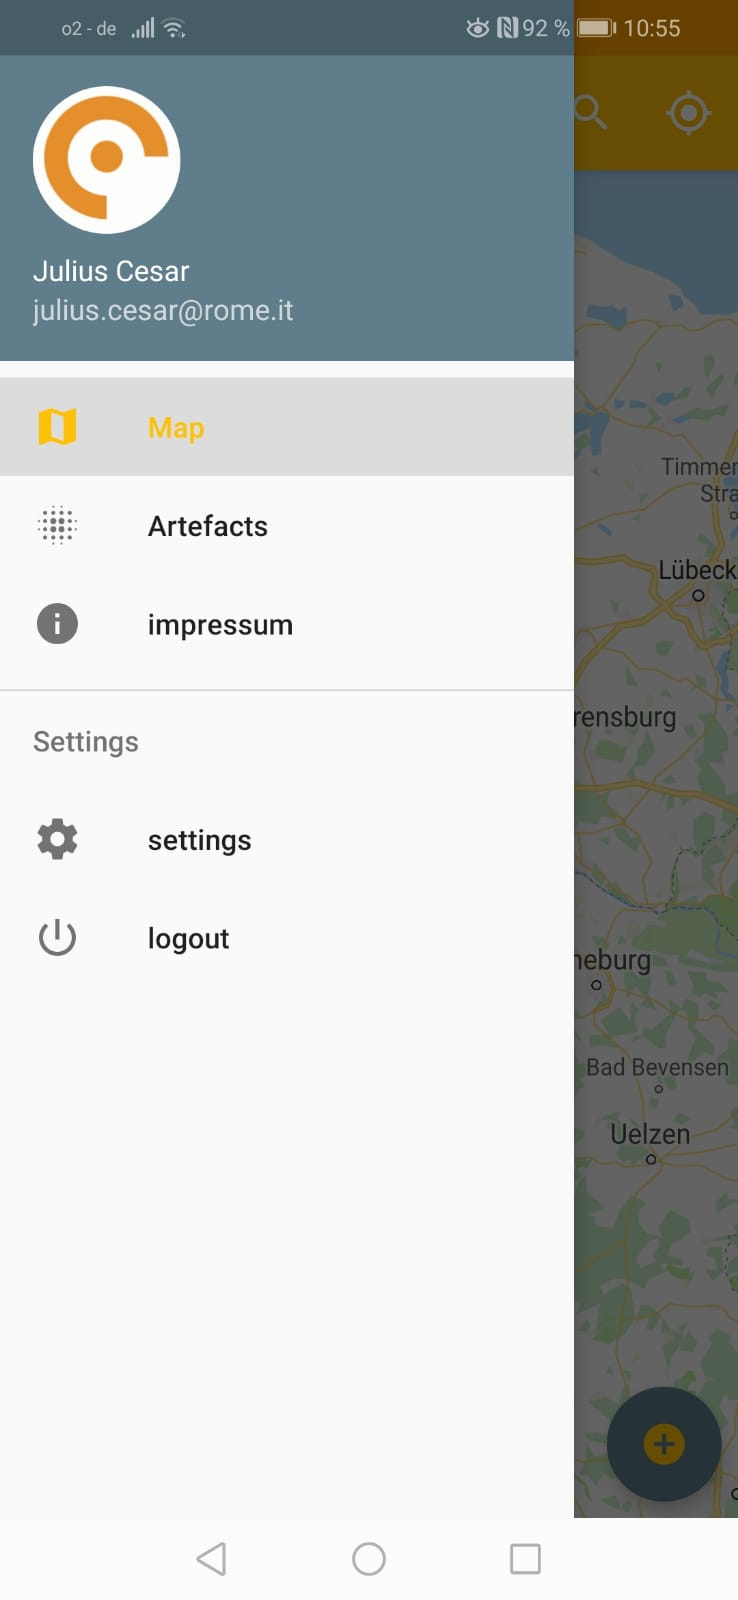
\includegraphics[width=\linewidth]{realization/realization_drawer.png}
  \caption{Navigation Drawer}\label{fig:realization_drawer}
\endminipage\hfill
\end{figure}

The list of options is not fixed to a precise account of items, so it can be extended during the next development period if new requirements occur. Furthermore, the settings option is a placeholder yet; it would be appreciated if it were implemented in the future.


% ################## FILTER ######################

\subsection{Filter}
As mentioned above, the filter menu was a complex part of the app. Since the old Civitas app allows the user to filter by date and category in a determinate way on the map, the new version extends the filtering by another dimension, the artefact list overview within the ArtefactListFragment. According to the user's habits, the user expects the filter settings to remain valid until they were reset, whether one is at the MapActivity or the ArtefactListFragment. Further, one switches between them with the expectation to get the same output results. Therefore, one has to save the current filter settings and check them in each of the mentioned parts. These are the GUI elements for the menu: CardView, RadioGroup, RadioButtons, EditText, Spinner, and Buttons. 
The RadioGroup allows a user to select one of the possible options. Selecting one option enables the corresponding elements in its row, and disables the other elements. One can choose to filter by date, and by category. If a filter parameter is applied, the \textbf{ResetFilter} Button and the \textbf{ShowSearchResult} Button becomes enabled. It is planned to expand the filter parameter by the property \textbf{OwnerId}, when this document is submitted, to satisfy the mentioned use-case. However, at the ArtefactListFragment is also a live filter search by artefact name available. Start typing instantly shows up with the matching filter results.
The filter menu is displayed in the following image set.

\begin{figure}[!htb]
\minipage{0.49\textwidth}
  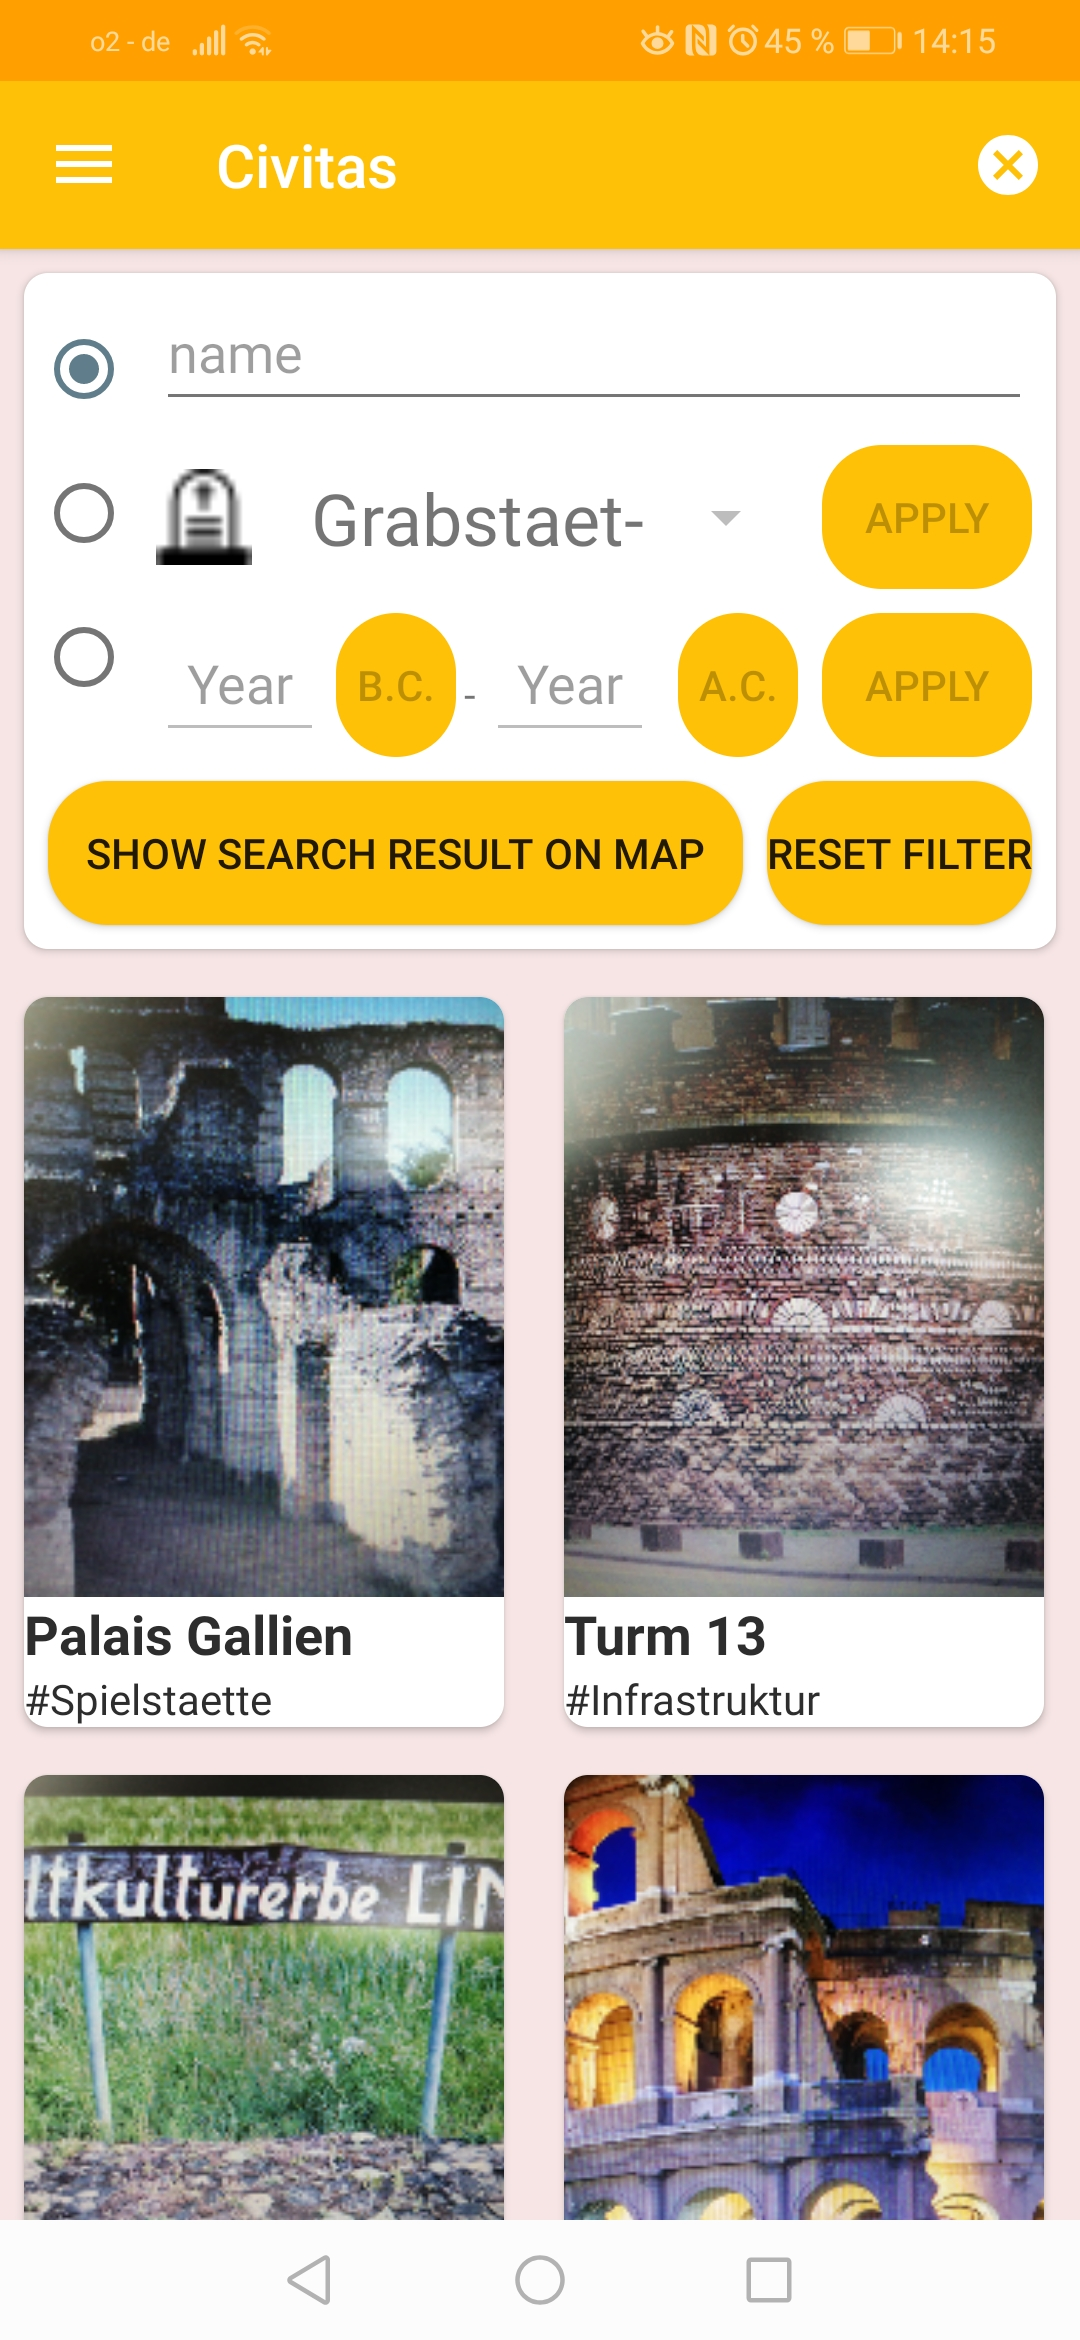
\includegraphics[width=\linewidth]{realization/realization_list_filter.png}
  \caption{Artefact list filter menu}\label{fig:awesome_image1}
\endminipage\hfill
\minipage{0.49\textwidth}
  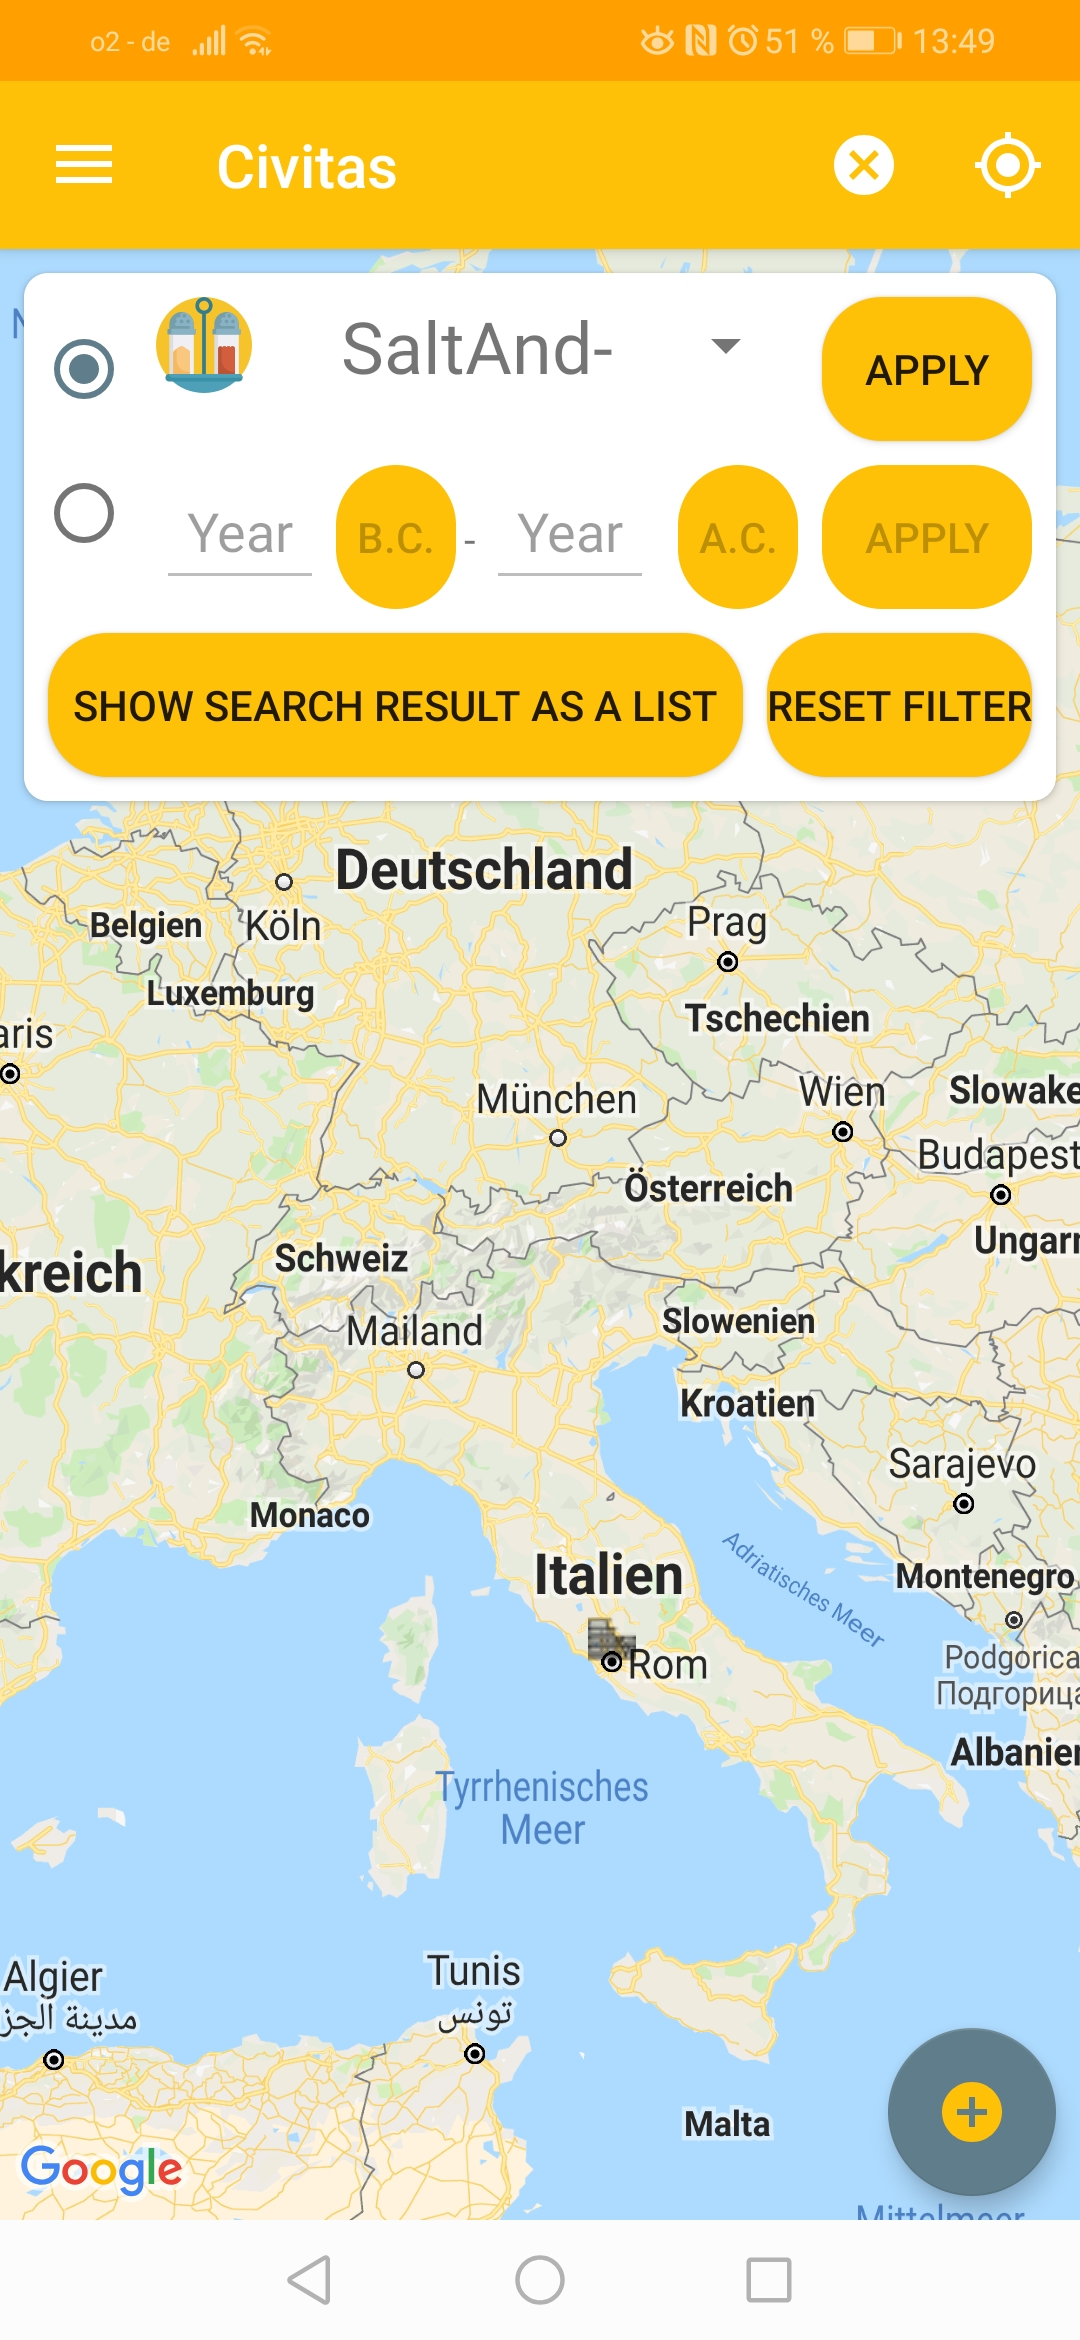
\includegraphics[width=\linewidth]{realization/realization_map_filter.png}
  \caption{Map filter menu}\label{fig:awesome_image2}
\endminipage\hfill
\caption{Filter general}
\label{fig:filter general}
\end{figure}









